% **********************************************************************
% LaTeX2e source for SensKINSOL user's guide.
% Last revised 30 August 2001 by Keith Eric Grant, LLNL
% **********************************************************************

\documentclass[11pt]{article}

\usepackage[dvips]{graphicx}
\usepackage{palatino}

\setlength{\oddsidemargin}{0in}
\setlength{\evensidemargin}{0in}
\setlength{\textwidth}{6.5in}

\newcommand{\thisdoc}{User Documentation for SensKINSOL, a Variant of
\\KINSOL for Sensitivity Analysis}

\newcommand{\writers}{Keith E. Grant, Alan C. Hindmarsh, and Allan
G. Taylor}

\title{\thisdoc %
\thanks{ This work was performed under the auspices of the U.S.
Department of Energy by University of California Lawrence Livermore
National Laboratory under contract No. W-7405-Eng-48.}}

\author{\writers %
\thanks{Center for Applied Scientific Computing, L-561, LLNL,
Livermore, CA 94551.}}

\begin{document}

\thispagestyle{empty}

% Generate cover page

% \vspace*{\fill}
\vspace*{0.1in}

\begin{center}

\LARGE
\thisdoc

\par\vspace*{0.7in}
\large
\writers
\par\bigskip\bigskip

{\em Lawrence Livermore National Laboratory}

\vspace{2in}
\par\large \today
\end{center}

\vfill
\mbox{}
\vfill
% \vspace*{3in}

% LLNL report info

\par\Large{\it Center for Applied Scientific Computing}
\vspace*{0.7in}
\par\large UCRL-??????

\newpage
\pagenumbering{roman}

% Disclaimer

\vspace*{0.25in}

\scriptsize
\begin{center}
\begin{minipage}{4.0in}

\begin{center}
DISCLAIMER
\end{center}

This document was prepared as an account of work sponsored by an agency
of the United States Government. Neither the United States Government
nor the University of California nor any of their employees, makes any
warranty, express or implied, or assumes any legal liability or
responsibility for the accuracy, completeness, or usefulness of any
information, apparatus, product, or process disclosed, or represents
that its use would not infringe privately owned rights. Reference
herein to any specific commercial product, process, or service by trade
name, trademark, manufacturer, or otherwise, does not necessarily
constitute or imply its endorsement, recommendation, or favoring by the
United States Government or the University of California. The views and
opinions of authors expressed herein do not necessarily state or
reflect those of the United States Government or the University of
California, and shall not be used for advertising or product
endorsement purposes.

\medskip
This work was performed under the auspices of the U.S. Department of
Energy by University of California Lawrence Livermore National
Laboratory under contract No. W-7405-Eng-48.
\end{minipage}
\end{center}
\normalsize

% End of cover/disclaimer pages

\newpage
\begin{center}
\LARGE
\thisdoc
\par\bigskip\medskip
\large
\writers
\par\bigskip\bigskip
\normalsize
\end{center}

\tableofcontents
\newpage
%
% \vspace*{2in}
% \begin{center}
% This Page Blank for Two-Sided Printing
% \end{center}
% \vfill
% \newpage
%
\maketitle
\pagenumbering{arabic}
\setcounter{page}{1}
\setlength{\parindent}{0pt}
\setlength{\parskip}{1.5ex plus 0.5ex minus 0.2ex}

\section{Introduction}

SensKINSOL is an extension of KINSOL for solving both a nonlinear
system of equations and the sensitivity of the solution to variation
of system parameters. KINSOL is a general purpose nonlinear system
solver callable from either C or FORTRAN programs
\cite{KINSOLusrguide}. It is based on NKSOL \cite{BrSa90}, but is
written in ANSI-standard C rather than FORTRAN77.  Its most notable
feature is that it uses Krylov Inexact Newton techniques in the
system's approximate solution, thus sharing significant modules
previously written within CASC (Center for Applied Scientific
Computing) at LLNL to support CVODE \cite{CoHi94,CoHi96} and PVODE
\cite{LDRD98,PVODEusrguide,ByHi99}.

On top of the KINSOL nonlinear solver framework, SensKINSOL adds the
additional linear solver framework required for estimating the
sensitivity of the solution of a nonlinear system to variations in
individual system parameters. Like KINSOL, SensKINSOL is written in C
and maintains the ability to be called from either C or FORTRAN. If the
solution to the system object function is known {\it a priori},
SensKINSOL provides an interface for accepting and verifying the
solution without calling the nonlinear solver.

Compared to direct methods, KINSOL and thus SensKINSOL require almost
no matrix storage for solving the Newton equations. The name
\mbox{KINSOL} is derived from those techniques: Krylov Inexact Newton
SOLver. The SensKINSOL package is arranged so that selecting one of two
forms of a single module in the compilation process will allow the
entire package to be created in either sequential (serial) or parallel
form. The parallel version of SensKINSOL uses MPI (Message-Passing
Interface) \cite{MPI} and the parallel version of the vector module
{\em NVECTOR}, discussed in Sections \ref{subsec:SolvingNonlin} and
\ref{subsec:SupportMod}, to achieve parallelism and portability.
SensKINSOL in parallel form is intended for the SPMD (Single Program
Multiple Data) model with distributed memory, in which all vectors are
identically distributed across processors. In particular, the vector
module {\em NVECTOR} is designed to help the user assign a contiguous
segment of a given vector to each of the processors for parallel
computation.

The remainder of this paper is organized as follows: Section 2 sets
the mathematical notation and summarizes the basic methods for
SensKINSOL. Section 3 summarizes the organization of the SensKINSOL
solver, while Section 4 summarizes its usage.  Section 5 describes a
preconditioner module, Section 6 describes a set of FORTRAN/C
interfaces, Section 7 describes an example problem, and Section 8
discusses availability.


\section{Mathematical Considerations}
\subsection{Solving the nonlinear system with SensKINSOL}
\label{subsec:SolvingNonlin}

SensKINSOL interfaces to KINSOL \cite{KINSOLusrguide} to solve the
nonlinear system of N equations
\begin{equation}
F(u) = 0, \label{nonlinear system}
\end{equation}
where $F(u)$ is a nonlinear function from ${\bf R}^N$ to ${\bf R}^N$.
An Inexact Newton method is applied to (\ref{nonlinear system})
resulting in the following algorithm:
\begin{quote}
{\bf Inexact Newton iteration}
\begin{enumerate}
   \item Set $u_0 = $ an initial guess
   \item For $n = 0, 1, 2,...$ until convergence do:\nonumber
      \begin{itemize}
          \item[(a)] Solve $J(u_n)\delta_n = - F(u_n) + r_n$
          \item[(b)] Set $u_{n+1} = u_n + \delta_n$
          \item[(c)] Test for convergence
      \end{itemize}
\end{enumerate}
\end{quote}
Here, $J(u_n) = F'(u_n)$ is the system Jacobian. As SensKINSOL and
KINSOL were designed for use on large systems, only iterative methods
were considered to solve the system in step 2(a). The solution is
approximate, with the linear residual $r_n$ being made to satisfy a
heuristic tolerance test determined for each nonlinear step
\cite{EiWa96}. Methods of this type used for solution of nonlinear
systems are called Inexact Newton methods. At each stage in the
iteration process, a multiple of the approximate solution $\delta_n$ to
the equation of step 2(a) is applied to the previously determined
iterated approximate solution to produce a new approximate solution.
Convergence is tested before iteration continues. The iterative method
currently implemented is one of the class of Krylov methods.

As only the matrix-vector product $J(u)v$ is required in the Krylov
method, in this nonlinear equations setting that action is approximated
by a difference quotient of the form
\begin{equation}
    J(u)v  \approx \frac {F(u+\sigma v) - F(u)}{\sigma},  \label{jacobv}
\end{equation}
where $u$ is the current approximation to a root of (\ref{nonlinear
system}) and $\sigma$ is a scalar, appropriately chosen to minimize
numerical error in the computation of (\ref{jacobv}). An optional
user-defined routine implementing this matrix-vector product is
accommodated. See further details in Section
\ref{subsubsec:DescSensKINSpgmr} describing the routine {\em
SensKINSpgmr}.

To the above methods are added scaling and preconditioning. Scaling is
allowed for both the approximate solution vector and the system
function vector. Additionally, right preconditioning is provided for if
the preconditioning setup and solve routines are supplied by the user.

While only one linear solver is now implemented for use with this
package, the formal structure is in place for alternate solvers. The
solver currently implemented is the GMRES solver \cite{BrHi89,SaSc86}
in module {\em Spgmr} and accessed via {\em SensKINSpgmr}. Here GMRES
stands for Generalized Minimal RESidual and SPGMR stands for Scaled
Preconditioned GMRES. In most cases, performance of SPGMR is improved
by user-supplied preconditioners.

SPGMR is one of a class of preconditioned Krylov methods.  Write the
linear system  simply as
\begin{equation}
 A x = b . \label{Linsys}
\end{equation}
A preconditioned Krylov method for (\ref{Linsys}) involves a
preconditioner matrix $P$ that approximates $A$, but for which
linear systems $Px=b$ can be solved easily.  For preconditioning
on the right, the Krylov method is applied to the equivalent system
\begin{equation}
 (A P^{-1}) (P x) = b .
\end{equation}
In SensKINSOL, the user may precondition the system on the right or use
no preconditioner. Two scalings are also provided for the system, one
to $F$ (hence the vector $b$) and one to $u$ (hence the vector $x$).
With these and the preconditioning combined, the Krylov method (in our
case GMRES) is applied to the transformed system

\begin{equation}
 \bar{A} \bar{x} = \bar{b} .
\end{equation}
From an initial guess $\bar{x}_0$, an approximate solution $\bar{x}_m
= \bar{x}_0 + z$ is obtained for $m = 1, 2, \ldots$ (until
convergence), with $z$ chosen from the Krylov subspace $K_m =
span\{r_0, \bar{A}r_0, \ldots, \bar{A}^{m-1}r_0\}$ of dimension $m$,
where $r_0$ is the initial residual $\bar{b} - \bar{A} \bar{x}_0$.
Each Krylov iteration requires one matrix-vector multiply operation
$\bar{A} v$, which is a combination of multiplies by $A$ and by
$P^{-1}$.  Multiplication of a given vector $v$ by $A$ requires the
product $Jv$, and that is approximated by a difference quotient
$[F(u+\sigma v) - F(u)]/\sigma$. Multiplication by $P^{-1}$ is to be
provided by the user of the solver, and is generally problem-dependent.
In the case of GMRES, the choice in $K_m$ is based on minimizing the
$L_2$ norm of the residual $\bar{b} - \bar{A} \bar{x}_m$
\cite{BrHi89,SaSc86}. When a given $\bar{x}_m$ meets the linear system
convergence criterion, $\bar{x}_m$ corresponds to the next increment
$\delta_n$ in the solution of (\ref{nonlinear system}) : $\delta_n$ is
obtained from $\bar{x}_m$ by applying scaling and preconditioning. The
increment $\delta_n$ is then added to $u_n$ to form $u_{n+1}$ in step
2(b) by one of the strategies discussed below. The new iterate
$u_{n+1}$ is tested for (nonlinear) convergence in (\ref{nonlinear
system}) , which is step 2(c) of the Inexact Newton iteration.

Two methods of applying a computed step $\delta_n$ to the previously
computed approximate solution vector are implemented. Denoted 'global
strategies', they attempt to use the direction implied by $\delta_n$ in
the most efficient way in furthering convergence of the global (i.e.,
nonlinear) problem. The first and simplest is the Inexact Newton
strategy.  A more advanced technique is implemented in the second
strategy, called Linesearch. The so-called 'Forcing Term' algorithms of
Eisenstat and Walker \cite{EiWa96} to control the linear convergence
tolerance are also implemented.

A fundamental set of mathematical operations on $N$-vectors has been
written for both CVODE/\linebreak[0]PVODE and
KINSOL/\linebreak[0]SensKINSOL. This set of computational kernels
exists in a distinct code module called {\em NVECTOR}. By separating
these frequent operations from the rest of the code, almost all
operations in SensKINSOL with significant potential for parallel
computation have been isolated. Then, two different sets of kernels,
both with the same routine names and a common interface, allow
parallel computation to be very simply implemented in these codes. The
operations done by this set of kernels are vector addition, scaling,
and copy, vector norms, scalar products, and so forth.

\subsection{Solving for parameter sensitivity with SensKINSOL}
\label{subsec:SolvingSens}

In considering the sensitivity analysis of (\ref{nonlinear system}), we
now assume that there is a set of $M$ parameters $p$ such that, given
$p$, we solve the system
\begin{equation}
F(u,p) = 0, \label{sensitivity system}
\end{equation}
for $u$. Considering the effect of varying $p$ while requiring that
(\ref{sensitivity system}) continues to be satisfied yields
\begin{equation}
\frac{{dF}}{{dp}} = \frac{{\partial F}}{{\partial u}}\frac{{\partial
u}}{{\partial p}} + \frac{{\partial F}}{{\partial p}} = 0
\label{sensvariation}
\end{equation}

We can now write the linear system
\begin{equation}
J\,s =  - \frac{{\partial F}}{{\partial p}} \label{eq_sens}
\end{equation}

where $J$ is the Jacobian of the original system of (\ref{sensitivity
system}) and $s$ are the sensitivity solutions. There are potential
practicality problems in using (\ref{eq_sens}) as the units and
magnitudes of the sensitivities $s$ do not match those of $u$ nor are
they necessarily similar from parameter to parameter. One remedy is to
scale the sensitivities by the nominal magnitude of the corresponding
parameters. Introducing the nominal parameter magnitudes $\bar{p}$, we
write the scaled sensitivities

\begin{equation}
w = \bar p\, s = \bar p\, \frac{{\partial u}}{{\partial p}} . \label{scaled sens}
\end{equation}

We can then rewrite (\ref{eq_sens}) as

\begin{equation}
J\,w =  - \bar p\, \frac{{\partial F}}{{\partial p}} .
\end{equation}

For those familiar with the inclusion of forward in time (i.e. tangent
linear) sensitivity analysis for a time-dependent system of ODEs or
DAEs, we note that sensitivity analysis of a nonlinear system is
simpler. Most significant to the structuring of SensKINSOL is that the
sensitivity analysis is a linear problem done as a post-process to the
nonlinear solution rather than as a concurrent solution.

The sensitivity analysis for the system (\ref{sensitivity system})
separates into $M$ separate problems for vectors of length $N$ --- one
for each scalar parameter. Because $J$ is the same for all $M$
problems, the preconditioning is done once and saved. Rather than
storing the entire $M\times N$ sensitivity solution array, a user may
only be interested in accumulating the action of each $N$ vector.
Accordingly, the SensKINSOL interface is designed to solve for the
sensitivity of $u$ to a single parameter at a time, giving the user
control of whether the sensitivity vectors are stored or applied
immediately. Under this assumption that only a single parameter is
being varied at a time, (\ref{scaled sens}) can be approximated by one
of

\medskip
\begin{equation}
\bar p\frac{{\partial F}}{{\partial p}}\quad  \cong \quad
\left\{\begin{array}{*{20}c}
   {\bar p\frac{\displaystyle{F(u,p + \Delta p) - F(u,p)}}{{\Delta p}}\quad ,} \hfill  \\
   \\
   {\bar p\frac{\displaystyle{F(u,p) - F(u,p - \Delta p)}}{{\Delta p}}\quad {\rm or}} \hfill  \\
   \\
   {\bar p\frac{\displaystyle{F(u,p + {{\Delta p} \mathord{\left/
 {\vphantom {{\Delta p} 2}} \right.
 \kern-\nulldelimiterspace} 2}) - F(u,p - {{\Delta p} \mathord{\left/
 {\vphantom {{\Delta p} 2}} \right.
 \kern-\nulldelimiterspace} 2})}}{{\Delta p}}} \hfill  \\
\end{array}\right\}
\end{equation}

\bigskip
where
\begin{equation}
\Delta p = sign(p)\;\bar p\;\zeta \;\sqrt \varepsilon \label{delta param}
\end{equation}
\smallskip

$\varepsilon$ is the error tolerance for the evaluation of $F$, and
$\zeta$ is a user chosen positive scaling factor having the nominal
magnitude of one. Apart from the user factor, the choice of parameter
step size given by (\ref{delta param}) has been made to minimize the
order of error in the evaluated derivative \cite[pp. 79-80]{Kelley95}.


\section{Code Organization}
\subsection{The User Module}

As is shown in \mbox{Fig. \ref{senskin struct}}, SensKINSOL is
organized into layers. A module's name is used to indicate the general
function of the module's contents. The user's main program is at the
top level. This routine, with other user-supplied routines, makes
various initialization calls, manages input/output, and calls the {\em
SensKINSOL} kernel module which carries out the solution of the
nonlinear system. The user module also defines and initializes {\em
f\_data}, the user data structure, via which SensKINSOL conveys current
parameter values to the user object function ({\em func}).

\begin{figure}
\begin{center}
\includegraphics[width=4.5in]{senskin_struct.eps}
\caption{Overall structure of the SensKINSOL package. Modules comprising
the central solver are indicated by boxes with rounded corners. Kernel
modules for SensKINSOL are shown on a solid gray background. Modules on
the octagon tiling are specific to the use of a particular linear solver
package --- currently SPGMR. Modules on the brick tiling provide more
general math and parallelization support} \label{senskin struct}
\end{center}
\end{figure}

\subsection{SensKINSOL Kernel Modules}

At the second level, are the interface modules {\em SensKINSOL} and
{\em SensKINSpgmr}. The {\em SensKINSOL} module calls the {\em KINSOL}
kernel module which controls the iterative nonlinear solution process.
The {\em SensKINSOL} and {\em KINSOL} modules comprise the SensKINSOL
kernel (\mbox{Fig. \ref{senskin struct}}, solid gray background) and
both are independent of the linear system method. The {\em SensKINSOL}
module also contains the routines called by the user program to perform
the linear solutions for the parameter sensitivity problems. In solving
these sensitivity problems, {\em SensKINSOL} calls a linear solver
wrapper within {\em KINSpgmr}. The \mbox{\em SensKINSpgmr} module
exists solely to provide the user's main routine an interface,
consistent with {\em SensKINSOL}, for initializing the underlying {\em
KINSpgmr} module. \mbox{\em SensKINSOL}, \mbox{\em KINSOL}, {\em
SensKINSpgmr}, and {\em KINSpgmr}, all shown in \mbox{Fig. \ref{senskin
struct}} with rounded boxes, comprise the SensKINSOL central solver.

\subsection{The Linear Solver Modules}

In solving the nonlinear system, {\em KINSOL} calls the user-supplied
function $F$, known as {\em func} internally, and accesses the linear
system solver (\mbox{Fig. \ref{senskin struct}}, octagonal tiling). At
the third level is found the linear system solver {\em KINSpgmr}, which
provides {\em KINSOL's} interface to a generic solver for the SPGMR
method, consisting of modules {\em Spgmr} and {\em Iterative}. {\em
KINSpgmr} also provides the linear solver wrapper used for parameter
sensitivity solutions. It accesses the user-supplied preconditioner
solve routine {\em Psolve}, if specified, and, if supplied, accesses a
user-supplied routine {\em Precondset} that computes and preprocesses
the preconditioner. The {\em Precondset} routine is usually implemented
by way of an approximate Jacobian matrix. Other linear system solvers
may be added to the package in the future. Such additions will be
independent of the {\em SensKINSOL} and {\em KINSOL} modules. The {\em
SensKINSpgmr} and {\em KINSpgmr} modules will only require
modification to default routines in a manner largely transparent to
the user.

\subsection{Support Modules and Parallelization}
\label{subsec:SupportMod}

Several supporting modules reside at the fourth level (Fig.{
}\ref{senskin struct}, brick tiling). These include {\em LLNLTYPS},
{\em LLNLMATH}, and {\em NVECTOR}. The first of these defines types
{\em real} and {\em integer}. The second specifies power functions, and
the third is discussed further below.

The key to being able to move from the sequential computing environment
to the parallel computing environment lies in the {\em NVECTOR} module.
This module was briefly mentioned in the previous section. The idea is
to distribute solution of the nonlinear system over several processors
so that each processor is solving a contiguous subset of the system.
This is achieved through the {\em NVECTOR} module, which handles all
calculations on $N$-vectors in a distributed manner, when the parallel
version is compiled with parallel libraries. For any vector operation,
each processor performs the operation on its contiguous elements of the
input vectors, of length (say) {\em Nlocal}, followed by a global
reduction operation where needed. In this way, vector calculations can
be performed simultaneously with each processor working on its block of
the vector. Vector kernels are also designed to be used in a
straightforward way for various vector operations that require the use
of the entire distributed $N$-vector.  These kernels include dot
products, various norms, linear sums, and so on.

The key to simply handling both parallel and serial applications of a
code lies in standardizing the interface to the vector kernels: both
sequential and parallel versions of {\em NVECTOR} have an identical
interface. In this way, one can access the kernels without referring
directly to the underlying vector structure. This is assisted by using
abstract data types that describe the machine environment data block
({\em type machEnvType}) and all $N$-vectors ({\em type N\_Vector}).
Functions to define a block of machine-dependent information and to
free that block of information are also included in the vector module.
Because the KINSOL interface to the vector kernels is independent of
the vector structure, the user could supply their own kernel to best
fit their application data structures. All references to parallelism
are in the kernel, thus, the user would handle all parallel aspects in
this case.

The parallel version of KINSOL uses the MPI (Message Passing Interface)
system \cite{MPI} for all inter-processor communication. This achieves
a high degree of portability, since MPI is becoming widely accepted as
a standard for message passing software. For a different parallel
computing environment, some rewriting of the vector module could allow
the use of other specific machine-dependent instructions.

\subsection{SensKINSOL Memory and Data Organization}

\mbox{Figure \ref{mem structs}} displays the essential data structures
used to implement SensKINSOL. The user must allocate and initialize the
parameter array $p$ and parameter magnitude array $\bar{p}$. These
arrays were previously defined in Section \ref{subsec:SolvingSens} in
describing Equations (\ref{sensitivity system}), (\ref{sensvariation}),
(\ref{scaled sens}) and (\ref{delta param}). The array $p$ contains the
parameters of the system object function of (\ref{sensitivity system}).
The arrary $\bar p$ provides nominal magnitudes of the parameters that
are used for the sensitivity scaling defined in (\ref{scaled sens}).
Pointers to these arrays along with other information are initialized
in the {\em Sensitivity Memory} structure via a call to SensKINMalloc
(see Section \ref{subsubsec:DescSensKINMalloc}). The user must also
place a pointer to $p$ in the {\em User Data} Structure (f\_data), so
that the user's system object function will have access to the
parameters as they are varied by SensKINSOL according to
(\ref{delta param}).

\begin{figure}
\begin{center}
\includegraphics[width=4.5in]{sens_kinsol_data_bw.eps}
\caption{SensKINSOL Memory and Data Organization. Note that pointers to
the user's parameter array must be present in {\bf both} the {\em User
Data} structure (f\_data) and in the {\em Sensitivity Memory}
structure.} \label{mem structs} \end{center} \end{figure}


\section{Using SensKINSOL}
\subsection{Overview}

We now turn to describing the sequence of calls to routines necessary
to use SensKINSOL. These are shown and compared with those required
for standard KINSOL in \mbox{Table \ref{callseq}}. One essential
prerequisite for the sensitivity analysis framework to work is that
the user both place a pointer to the parameter array $p$
(\ref{sensitivity system}) in the {\em User Data} structure and pass a
pointer to the same array to SensKINMalloc where it is placed in the
{\em Sensitivity Memory} structure (\mbox{Fig. \ref{mem structs}}). By
this mechanism, the $p$ array is available to both SensKINSOL and the
system object function. Thus, when SensKINSOL varies a parameter
according to Equation (\ref{delta param}), the change will be visible
to the object function $func$. Implicit within this, is the
requirement that the user has allocated and initialized the parameter
array $p$ and parameter magnitude array $pbar$ in the main program
before initializing SensKINSOL.

\begin{table}
\caption{Comparision of KINSOL and SensKINSOL Call Sequences} \label{callseq}
\begin{center}
\begin{tabular}{|l|l|}
\hline
 & \\
KINMalloc & SensKINMalloc \\
Allocate and initialize UserData  & Allocate and initialize UserData \\
KINSpgmr & SensKINSpgmr \\
KINSOL  & SensKINSOL or SensKINInit \\
  & SensKINLinInit \\
  & Loop over parameters \{ \\
  & \hspace{2em}SensKINDiff (optional) \\
  & \hspace{2em}SensKINLinSolve \\
  & \} \\
KINFree & SensKINFree \\
Deallocate UserData  & Deallocate UserData \\
  & \\
\hline
\end{tabular}
\end{center}
\end{table}

\subsection{Detailed Descriptions of Routines}
This subsection contains extracts from header files for SensKINSOL
(\mbox{\em sens\_kinsol.h}) and SensKINSpgmr (\mbox{\em
sens\_kinspgmr.h}) detailing the arguments of user-callable routines.
For each routine, the declaration with arguments is followed by a
section of comments from the corresponding section of the appropriate
header file. Please note the the system function $F(u)$ is called
$func(uu)$ in the SensKINSOL and SensKINSpgmr source code. Also, the
system solution variable $u$ is called $uu$ in coding for these
modules. Note also that the routines SensKINSOL and SensKINInit have
the same calling arguments. The difference between these two routines
is that SensKINInit assumes that the solution $u$ to the system
function is already known.

\subsubsection{SensKINMalloc --- Memory allocation and initialization}
\label{subsubsec:DescSensKINMalloc}
\small
\begin{verbatim}
void *SensKINMalloc(integer Neq, integer np, integer diffrhs,
   real diffscl, real *p, real *pbar, FILE *msgfp, void *machEnv);

/**********************************************************************
 * Function : SensKINMalloc                                           *
 *                                                                    *
 * SensKINMalloc allocates and initializes a sensitivity parameter    *
 * structure                                                          *
 *--------------------------------------------------------------------*
 *                                                                    *
 * Arguments...                                                       *
 *                                                                    *
 * Neq      size of vectors being handled by the current memory       *
 *          allocation call to SensKINMalloc                          *
 *                                                                    *
 * np       The number of sensitivity parameters (np >= 0)            *
 *                                                                    *
 * diffrhs  Determines the form of the RHS difference equation        *
 *             = DIFF_FRWRD = 0 : Forward difference                  *
 *             = DIFF_BKWRD = 1 : Backward difference                 *
 *             = DIFF_CNTRD = 2 : Centered difference                 *
 *                                                                    *
 * diffscl  Positive scale factor for the RHS difference increment.   *
 *          The nominal value for diffscl is 1.0                      *
 *                                                                    *
 * p        Array of sensitivity parameters of length np. The user    *
 *          should also place a pointer to this array within the      *
 *          f_data structure passed by KINSOL to the object function. *
 *                                                                    *
 * pbar     Array of sensitivity parameter nominal magnitudes > 0     *
 *                                                                    *
 * msgfp    Pointer to the file for error message output              *
 *                                                                    *
 * machEnv  A pointer to machine environment-specific information.    *
 *          Pass NULL for the sequential case (see nvector.h).        *
 *                                                                    *
 *                                                                    *
 * Return values...                                                   *
 *                                                                    *
 * SensKINMalloc =   Pointer to sensitivity memory. NULL on error     *
 *                                                                    *
 **********************************************************************/
\end{verbatim}
\normalsize

\subsubsection{SensKINSpgmr --- Linear solver initialization}
\label{subsubsec:DescSensKINSpgmr}
\small
\begin{verbatim}
int SensKINSpgmr(void *sens_params, int maxl, int maxlrst, int msbpre,
	      KINSpgmrPrecondFn precondset,
	      KINSpgmrPrecondSolveFn psolve,
	      KINSpgmruserAtimesFn userAtimes,
         void *P_data);

/**********************************************************************
 *                                                                    *
 * Function: SensKINSpgmr                                             *
 *                                                                    *
 * This routine encapsulates a call to KINSpgmr. The arguments are    *
 * the same as for KINSpgmr except that a pointer to a sensitivity    *
 * memory structure is passed to SensKINSpgmr instead of a pointer    *
 * to KINSOL memory.                                                  *
 * -------------------------------------------------------------------*
 *                                                                    *
 * sens_params    Pointer to a sensitivity memory structure that      *
 *                contains a pointer to the KINSOL memory             *
 *                                                                    *
 * ...            See kinsol.h and the KINSOL user's guide            *
 *                                                                    *
 **********************************************************************/
\end{verbatim}
\normalsize

\subsubsection{SensKINSOL --- Solving the nonlinear system}
\small
\begin{verbatim}
 int SensKINSOL(void *sens_params, integer Neq, N_Vector uu,
         SysFn func, int globalstrategy, N_Vector uscale,
         N_Vector fscale, real fnormtol, real scsteptol,
         N_Vector constraints, boole optIn, long int iopt[],
         real ropt[], void *f_data);

/**********************************************************************
 *                                                                    *
 * Function: SensKINSol                                               *
 *                                                                    *
 * This routine encapsulates a call to KINSOL. The arguments are      *
 * formally the same as for KINSOL except that a pointer to a         *
 * sensitivity memory structure is passed to SensKINSol instead of a  *
 * pointer to KINSOL memory. An additional underlying difference is   *
 * that the user's f_data structure must contain a pointer to the     *
 * same parameter array p[] that was passed to SensKINMalloc          *
 * -------------------------------------------------------------------*
 *                                                                    *
 * sens_params    Pointer to a sensitivity memory structure that      *
 *                contains a pointer to the KINSOL memory             *
 *                                                                    *
 * ...            See kinsol.h and the KINSOL user's guide            *
 *                                                                    *
 **********************************************************************/

\end{verbatim}
\normalsize

\subsubsection{SenKINInit --- Using a known solution for the nonlinear
system}
\small
\begin{verbatim}
int SensKINInit (void *sens_params, integer Neq, N_Vector uu,
        SysFn func, int globalstrategy, N_Vector uscale,
        N_Vector fscale, real fnormtol, real scsteptol,
        N_Vector constraints, boole optIn, long int iopt[],
        real ropt[], void *f_data);

/**********************************************************************
 * Function: SensKINInit                                              *
 *                                                                    *
 * This routine initializes KINSOL system variables needed by         *
 * SensKINSOL without calling the nonlinear solver. SensKINInit is    *
 * to be used when the solution uu of the nonlinear system F(uu) = 0  *
 * is already accurately known. At the cost of including some unused  *
 * variables (as noted below), the calling sequence to SensKINInit    *
 * has been kept the same as that to SensKINSOL                       *
 *                                                                    *
 * Arguments...                                                       *
 *                                                                    *
 *    sens_params       Pointer to the sensitivity memory structure   *
 *                                                                    *
 *    Neq               The number of equations in the algebraic      *
 *                      system                                        *
 *                                                                    *
 *    uu                Known solution for the system func(uu)=0.     *
 *                                                                    *
 *    func              Objective function for the system func(uu)=0. *
 *                                                                    *
 *    globalstrategy    Unused, but set to zero in KINSOL memory      *
 *                                                                    *
 *    uscale            An array (type N_Vector) of diagonal elements *
 *                      of the scaling matrix for uu. The elements of *
 *                      uscale must be positive values. The scaling   *
 *                      matrix uscale should be chosen so that        *
 *                      uscale * uu (as a matrix multiplication)      *
 *                      should have all its components with roughly   *
 *                      the same magnitude when uu is close to a root *
 *                      of func.                                      *
 *                                                                    *
 *    fscale            An array (type N_Vector) of diagonal elements *
 *                      of the scaling matrix for func. the elements  *
 *                      of fscale must be positive values. The        *
 *                      scaling matrix fscale should be chosen so     *
 *                      that fscale * func(uu) (as a matrix           *
 *                      multiplication) should have all its           *
 *                      components with roughly the same magnitude    *
 *                      when uu is NOT too near a root of func.       *
 *                                                                    *
 *    fnormtol          A real (scalar) value containing the stopping *
 *                      tolerance on maxnorm( fscale * func(uu) ). If *
 *                      fnormtol is input as 0., then a default value *
 *                      of (uround) to the 1/3 power will be used.    *
 *                      uround is the unit roundoff for the machine   *
 *                      in use for the calculation. (see UnitRoundoff *
 *                      in the llnlmath module                        *
 *                                                                    *
 *    scsteptol         Unused by SensKINInit                         *
 *                                                                    *
 *    constraints       Unused by SensKINInit                         *
 *                                                                    *
 *    optIn             is a flag indicating whether optional inputs  *
 *                      from the user in the arrays iopt and ropt are *
 *                      to be used. pass FALSE to ignore all optional *
 *                      inputs and TRUE to use all optional inputs    *
 *                      that are present. Either choice does NOT      *
 *                      affect outputs in other positions of iopt     *
 *                      or ropt.                                      *
 *                                                                    *
 *    iopt              The user-allocated array (of size OPT_SIZE)   *
 *                      that will hold optional integer inputs and    *
 *                      outputs. The user can pass NULL if he/she     *
 *                      does not wish to use optional integer inputs  *
 *                      or outputs. If optIn is TRUE, the user should *
 *                      preset to 0 those locations for which default *
 *                      values are to be used. See Optional Inputs    *
 *                      and Outputs in kinsol.h                       *
 *                                                                    *
 *    ropt              The user-allocated array (of size OPT_SIZE)   *
 *                      that will hold optional real inputs and       *
 *                      outputs. The user can pass NULL if he/she     *
 *                      does not wish to use optional real inputs or  *
 *                      outputs. If optIn is TRUE, the user should    *
 *                      preset to 0.0 the optional input locations    *
 *                      for which default values are to be used. See  *
 *                      Optional Inputs and Outputs in kinsol.h       *
 *                                                                    *
 *    f_data            A pointer to work space for use by the user-  *
 *                      supplied function func. The space allocated   *
 *                      to f_data is allocated by the user's program  *
 *                      before the call to SensKINMalloc.             *
 *                                                                    *
 * Return values...                                                   *
 *                                                                    *
 * SensKINInit = -4   Sensitivity memory allocation failuse           *
 *             = -3   KINSOL linear solver memory allocation failure  *
 *             = -2   KINSOL input error (see error output file)      *
 *             = -1   KINSOL memory allocation failure                *
 *             = +1   Success flag for F(uu)==0 satisfied             *
 *                                                                    *
 * Note: The above return values are compatible with those returned   *
 * by SensKINSOL. If uu is not a solution, this will be returned as   *
 * an input error (-2) with an appropriate error message.             *
 *                                                                    *
 **********************************************************************/
\end{verbatim}
\normalsize

\subsubsection{SensKINLinInit --- Initializing for sensitivity
estimates}
\small
\begin{verbatim}
int SensKINLinInit (void *sens_params);

/******************************************************************
 *                                                                *
 * Function : SensKINLinInit                                      *
 *                                                                *
 * This routine calls the linear solver setup routine to insure   *
 * that the preconditioning is current                            *
 *----------------------------------------------------------------*
 *                                                                *
 * Arguments...                                                   *
 *                                                                *
 * sens_params  Pointer to the sensitivity memory structure       *
 *                                                                *
 * Return Values...                                               *
 *                                                                *
 * SensKINLINInit = 0  Success                                    *
 *                = 1  Pointer to sensitivity memory NULL         *
 *                = 2  Pointer to KINSOL memory NULL              *
 *                = 3  Error in Preconditioning Setup             *
 *                                                                *
 ******************************************************************/
\end{verbatim}
\normalsize

\subsubsection{SensKINDiff --- Resetting sensitivity differencing
options}

The use of {\em SensKINDiff} is optional, since the same differencing
option and scaling factor information are previously passed to
{\em SensKINMalloc}. What {\em SensKINDiff} allows is to change this
information between solving for the sensitivity of the system solution
to different parameters.

\small
\begin{verbatim}
int SensKINDiff (void *sens_params, integer diffrhs, real diffscl);

/******************************************************************
 *                                                                *
 * Function : SensKINDiff                                         *
 *                                                                *
 * What SensKINDIFF allows the user to do is to change the RHS    *
 * difference option and difference increment scaling factor      *
 * between the solutions for individual parameters. Use of        *
 * SensKINDiff is optional, since the user specifices values for  *
 * both diffrhs and diffscl in the call to SensKINMalloc          *
 *----------------------------------------------------------------*
 *                                                                *
 * Arguments...                                                   *
 *                                                                *
 * sens     Pointer to the SensKINSOL sensitivity structure       *
 *                                                                *
 *                                                                *
 * diffrhs  Determines the form of the RHS difference equation    *
 *             = DIFF_FRWRD = 0 : Forward difference              *
 *             = DIFF_BKWRD = 1 : Backward difference             *
 *             = DIFF_CNTRD = 2 : Centered difference             *
 *                                                                *
 * diffscl  Scale factor (positive) for the RHS difference        *
 *          increment. The nominal value for diffscl is 1.0       *
 *                                                                *
 * Return Values...                                               *
 *                                                                *
 * SensKINDiff = 0   Success                                      *
 *             = 1   Pointer to sensitivity memory NULL           *
 *             = 2   Difference scaling factor <= 0               *
 *             = 3   Differencing option not valid                *
 *                                                                *
 ******************************************************************/
\end{verbatim}
\normalsize

\subsubsection{SensKINLINSolve --- Solving for sensitivities}

Each call to {\em SensKINLINSolve} estimates the sensitivity of the
system solution $u$ to variation of a single system parameter.

\small
\begin{verbatim}
int SensKINLinSolve (void *sens_params, integer ip, N_Vector ww);

/******************************************************************
 *                                                                *
 * Function : SensKINLinSolve                                     *
 *                                                                *
 * This routine solves the linear system J w = v, where w is the  *
 * scaled sensitivity vector for the current parameter (ip) and   *
 * v = - pbar*partial(F)/partial(p).                              *
 *----------------------------------------------------------------*
 *                                                                *
 * Arguments...                                                   *
 *                                                                *
 * sens_params Pointer to the sensitivity memory structure        *
 *                                                                *
 * ip          Index of the current sensitivity parameter         *
 *                                                                *
 * ww          The sensitivity vector for parameter ip (returned) *
 *                                                                *
 *                                                                *
 * Return Values...                                               *
 *                                                                *
 * SensKINLinSolve:                                               *
 *                  = -10  Error in evaluating sensitivity RHS    *
 *                  =  -9  Pointer to sensitivity memory is NULL  *
 *                  =  -8  N_Vector for RHS is NULL               *
 *                  =  -7  N-Vector for solution is NULL          *
 *                  =  -6  Pointer to linear solver mem. is NULL  *
 *                  =  -5  Pointer to KINSOL memory is NULL       *
 *                  =  -4  Other unrecoverable failure            *
 *                  =  -3  Unrecoverable preconditioner error     *
 *                  =  -2  Unrecoverable ATimes routine error     *
 *                  =  -1  NULL pointer found by Krylov solver    *
 *                  =   0  A linear solver success story          *
 *                  =   1  Recoverable failure to converge        *
 *                  =   2  Recoverable preconditioner error       *
 *                  =   3  A singular matrix was encountered      *
 *                  =   4  Other recoverable failure              *
 *                  =   5  Out of range sens. parameter index     *
 *                                                                *
 ******************************************************************/
\end{verbatim}
\normalsize

\subsubsection{SensKINFree --- Free Sensitivty and KINSOL memory}
\small
\begin{verbatim}
void SensKINFree (void *sens_params);

/**********************************************************************
 *                                                                    *
 * Function : SensKINFree                                             *
 *                                                                    *
 * This routine deallocates the sensitivity structure memory and      *
 * calls KINFree to deallocate the KINSOL memory structure            *
 *--------------------------------------------------------------------*
 *                                                                    *
 * Arguments...                                                       *
 *                                                                    *
 * sens     Pointer to the sensitivity structure to free              *
 *                                                                    *
 **********************************************************************/
\end{verbatim}
\normalsize

\subsection{A Template of the User's Main Program}
\subsubsection{Template of required user program steps}

\begin{enumerate}

\item {\em MPI\_Init(\&argc, \&argv);} Called to initialize MPI if MPI
is used by the user's program.  Here, {\em argc} and {\em argv} are the
command line argument counter and array received by {\em main}.

\item Set {\em n}, the local vector length (the sub-vector length for
this processor); {\em Neq}, the global vector length (the problem size
$N$, and the sum of all the values of {\em n}); and the active set
of processors.

\item {\em machEnv = PVecInitMPI(comm, n, Neq, \&argc, \&argv);}
Initializes the parallel NVECTOR module.  Here, {\em comm} is the MPI
communicator, which may be set in one of two ways. If a proper subset
of active processors is to be used, {\em comm} must be set by suitable
MPI calls.  Otherwise, to specify that all processors are to be used,
{\em comm} must be {\em MPI\_COMM\_WORLD}.

\item Set the vector {\em u} of initial values.  Use the macro {\em
N\_VMAKE(u, udata, machEnv);} if an existing array {\em udata}
contains the initial values of $u$.  Otherwise, make the call {\em u =
N\_VNew(Neq, machEnv);} and load initial values into the array defined
by {\em N\_VDATA(u)}.

\item Allocate and initialize the arrays of system object function
parameters {\em p} and the nominal parameter magnitudes {\em pbar}.

\item {\em sensmem = SensKINMalloc(\ldots);} Allocates internal memory
for SensKINSOL and returns a pointer to the allocated SensKINSOL
memory structure.

\item {\em SensKINSpgmr(\ldots);} Initializes the {\em SPGMR} linear
solver.

\item {\em ier = SensKINSol(sensmem, u, \ldots );} Performs the nonlinear
solve or \\ {\em ier = SensKINInit(sensmem, u, \ldots );} Uses a known
solution to the nonlinear system.

\item {\em ier = SensKINLinInit (sensmem);} Initializes the linear
solver for the sensitivity solutions to follow.

\item {\em ier = SensKINDiff (sensmem, diffrhs, diffscl);} Changes the
sensitivity differencing option or difference scaling factor (optional
call)

\item {\em ier = SensKINLinSolve (sensmem, ip, ww);} Solves for the
scaled sensitivity {\em ww} of the system solution {\em uu} to the
{\em ip'th} parameter. Repeat for each parameter for which a
sensitivity is desired.

\item {\em N\_VDISPOSE;} or {\em N\_VFree;} Called upon completion of
all solutions to deallocate the memory for the vector {\em u},
allocated by {\em N\_VMAKE} or {\em N\_VNew}, respectively.

\item {\em SensKINFree(sensmem);} Frees the memory allocated for
SensKINSOL.

\item {\em PVecFreeMPI(machEnv);} Frees memory containing
machine-dependent data.

\end{enumerate}

\subsubsection{Summary of Serial Usage of SensKINSOL} \label{serial-usage}

\begin{enumerate}

\item {\em msgfile=fopen("***.out","w")}; Opens an output message
file, if desired.

\item Allocate and initialize user vectors and structures, as required.
These include {\em p} and {\em pbar}. A pointer to {\em p} must
also be placed in the user data structure ({\em f\_data}).

\item {\em sensmem = SensKINMalloc(Neq, np, \ldots);}

\item {\em ier = SensKINSpgmr(sensmem, \ldots);}

\item {\em ier = SensKINSol(sensmem, \ldots);} or \\
      {\em ier = SensKINInit(sensmem, \ldots);}

\item {\em ier = SensKINLinInit (sensmem);}

\item {\em ier = SensKINDiff (sensmem, diffrhs, diffscl);} (optional
call)

\item {\em ier = SensKINLinSolve (sensmem, ip, ww);} (repeat for each parameter)

\item {\em SensKINFree(sensmem);}

\item Deallocate user vectors and structures

\end{enumerate}

\subsubsection{Summary of Parallel Usage of SensKINSOL}
\label{parallel-usage}

\begin{enumerate}

\item {\em msgfile = fopen("***.out","w");} Opens an output message
file, if desired.

\item  {\em MPI\_Init();} Because {\em PVecInitMPI}, below, also calls
{\em MPI\_Init}, this call is only required if the user's program uses
MPI before step 3.

\item Set the NVECTOR local length {\em n}, NVECTOR global length {\em
Neq}, and the active set of processors.

\item
{\em machEnv = PVecInitMPI(comm, n, Neq, argc, argv);} \\
{\em comm = MPI communicator;} Communicators set up by the user, or \\
{\em comm} = {\em MPI\_COMM\_WORLD;} All processors specified, \\ 
{\em if (machEnv == NULL) return(1);}


\item {\em N\_VMAKE(u, udata, machEnv);} (If {\em udata} is an
existing data array) or \\ {\em u = N\_VNew(Neq,machEnv);} (If the
user sets up vectors, structures, etc).


\item  {\em sensmem = SensKINMalloc( Neq, np, \ldots);}


\item {\em ier = SensKINSpgmr(sensmem, \ldots);}

\item {\em ier = SensKINSol(sensmem, \ldots);} or \\
      {\em ier = SensKINInit(sensmem, \ldots);}


\item {\em ier = SensKINLinInit (sensmem);}

\item {\em ier = SensKINDiff (sensmem, diffrhs, diffscl);} Call optionally.

\item {\em ier = SensKINLinSolve (sensmem, ip, ww);} Repeat for each
parameter.

\item {\em SensKINFree(sensmem);}
\item {\em N\_VDISPOSE}(  ); or {\em N\_VFree}( ); Called, as appropriate.

\item {\em PVecFreeMPI(machEnv);} Frees memory containing
machine-dependent data.
\end{enumerate}

\subsubsection{Header files}

Every usage of SensKINSOL requires at least the inclusion of the
following header files: {\em senskinsol.h} and {\em kinsol.h}, and {\em
senskinspgmr.h}, {\em kinspgmr.h} or a future alternate linear solver,
{\em llnlmath.h}, {\em llnltyps.h}, and {\em nvector.h}. The header
file {\em mpi.h} is required for parallel applications of KINSOL.


\subsection{User-Supplied Functions}

The function defining the nonlinear system, called $F(u)$ in this
report, but {\em func(uu)} in {\em SensKINSOL} and {\em SensKINSpgmr}
internal usage, must be of the form described by the following typedef
extracted from {\em KINSOL}:

\small
\begin{verbatim}

typedef void (*SysFn)(integer Neq, N_Vector uu,
                  N_Vector fval,  void *f_data );

 /******************************************************************
 *                                                                *
 * Type : SysFn                                                   *
 *----------------------------------------------------------------*
 * The func function which defines the system to be solved :      *
 *              func(uu) = 0      must have type SysFn.           *
 * func takes as input the problem size Neq and the dependent     *
 * variable vector uu. The function stores the result of func(uu) *
 * in fval. The necessary work space, besides uu and fval,  is    *
 * provided by the pointer f_data.                                *
 * The uu argument is of type N_Vector.                           *
 * A SysFn function does not have a return value.                 *
 *                                                                *
 ******************************************************************/

\end{verbatim}
\normalsize

Preconditioning is an important step in using SenKINSOL with any linear
solver. The interface for the routines defining the preconditioner
setup and solve routines for {\em KINSPGMR} are given next.

\small
\begin{verbatim}

typedef int (*KINSpgmrPrecondFn)(integer Neq,
                 N_Vector uu, N_Vector uscale ,
                 N_Vector fval, N_Vector fscale,
                 N_Vector vtemp1, N_Vector vtemp2,
                 SysFn func, real uround,
                 long int *nfePtr, void *P_data);

/******************************************************************
 *                                                                *
 * Type : KINSpgmrPrecondFn                                       *
 *----------------------------------------------------------------*
 * The user-supplied preconditioner setup function precondset and *
 * the user-supplied preconditioner solve function precondsolve   *
 * together must define the right preconditoner matrix P chosen   *
 * so as to provide an easier system for the Krylov solver        *
 * to solve. precondset is called to provide any matrix data      *
 * required by the subsequent call(s) to precondsolve. The data is*
 * stored in the memory allocated to P_data and the structuring of*
 * that memory is up to the user.     More specifically,          *
 * the user-supplied preconditioner setup function precondset     *
 * is to evaluate and preprocess any Jacobian-related data        *
 * needed by the preconditioner solve function precondsolve.      *
 * This might include forming a crude approximate Jacobian,       *
 * and performing an LU factorization on the resulting            *
 * approximation to J.  This function will not be called in       *
 * advance of every call to precondsolve, but instead will be     *
 * called only as often as necessary to achieve convergence       *
 * within the Newton iteration in KINSOL.  If the precondsolve    *
 * function needs no preparation, the precondset function can be  *
 * NULL.                                                          *
 *                                                                *
 * precondset should not modify the contents of the arrays        *
 * uu or fval as those arrays are used elsewhere in the           *
 * iteration process.                                             *
 *                                                                *
 * Each call to the precondset function is preceded by a call to  *
 * the system function func. Thus the precondset function can use *
 * any auxiliary data that is computed by the func function and   *
 * saved in a way accessible to precondset.                       *
 *                                                                *
 * The two scaling arrays, fscale and uscale, and unit roundoff   *
 * uround are provided to the precondset function for possible use*
 * in approximating Jacobian data, e.g. by difference quotients.  *
 * These arrays should also not be altered                        *
 *                                                                *
 * A function precondset must have the prototype given below.     *
 * Its parameters are as follows:                                 *
 *                                                                *
 * Neq     is the length of all vector arguments.                 *
 *                                                                *
 * uu      an N_Vector giving the current iterate for the system. *
 *                                                                *
 * uscale  an N_Vector giving the diagonal entries of the uu-     *
 *         scaling matrix.                                        *
 *                                                                *
 * fval    an N_Vector giving the current function value          *
 *                                                                *
 * fscale  an N_Vector giving the diagonal entries of the func-   *
 *         scaling matrix.                                        *
 *                                                                *
 * vtemp1  an N_Vector temporary                                  *
 *                                                                *
 * vtemp2  an N_Vector temporary                                  *
 *                                                                *
 * func    the function func defines the system being solved:     *
 *         func(uu) = 0., and its name is passed initially to     *
 *         KINSOL in the call to KINMalloc                        *
 *                                                                *
 * uround  is the machine unit roundoff.                          *
 *                                                                *
 * nfePtr  is a pointer to the memory location containing the     *
 *           KINSOL problem data nfe = number of calls to func.   *
 *           The precondset routine should update this counter by *
 *           adding on the number of func calls made in order to  *
 *           approximate the Jacobian, if any.  For example, if   *
 *           the routine calls func a total of W times, then the  *
 *           update is *nfePtr += W.                              *
 *                                                                *
 * P_data is a pointer to user data - the same as the P_data      *
 *           parameter passed to KINSpgmr.                        *
 *                                                                *
 *                                                                *
 * Returned value:                                                *
 * The value to be returned by the precondset function is a flag  *
 * indicating whether it was successful.  This value should be    *
 *   0   if successful,                                           *
 *   1   if failure, in which case KINSOL stops                   *
 *                                                                *
 *                                                                *
 ******************************************************************/


typedef int (*KINSpgmrPrecondSolveFn)(integer Neq,
                 N_Vector uu, N_Vector uscale,
                 N_Vector fval, N_Vector fscale,
                 N_Vector vtem, N_Vector ftem,
                 SysFn func, real u_round,
                 long int *nfePtr, void *P_data);

/******************************************************************
 *                                                                *
 * Type : KINSpgmrPrecondSolveFn                                  *
 *----------------------------------------------------------------*
 * The user-supplied preconditioner solve function precondsolve   *
 * is to solve a linear system P x = r in which the matrix P is   *
 * the (right) preconditioner matrix P.                           *
 *                                                                *
 * precondset should not modify the contents of the iterate       *
 * array uu  or the current function value array  fval as those   *
 * are used elsewhere in the iteration process.                   *
 *                                                                *
 * A function precondsolve must have the prototype given below.   *
 * Its parameters are as follows:                                 *
 *                                                                *
 * Neq      is the length of all vector arguments.                *
 *                                                                *
 * uu      an N_Vector giving the current iterate for the system. *
 *                                                                *
 * uscale  an N_Vector giving the diagonal entries of the uu-     *
 *         scaling matrix.                                        *
 *                                                                *
 * fval    an N_Vector giving the current function value          *
 *                                                                *
 * fscale  an N_Vector giving the diagonal entries of the func-   *
 *         scaling matrix.                                        *
 *                                                                *
 * vtem    an N_Vector work array, holds the RHS vector on input  *
 *            and the result x on output/return                   *
 *                                                                *
 * ftem    an N_Vector work array, usually set on input as vtemp  *
 *                                                                *
 * func    the function func defines the system being solved:     *
 *         func(uu) = 0.                                          *
 *                                                                *
 * uround  is the machine unit roundoff.                          *
 *                                                                *
 * nfePtr is a pointer to the memory location containing the      *
 *          KINSOL problem data nfe = number of calls to func. The*
 *          precondsolve routine should update this counter by    *
 *          adding  on the number of func calls made in order to  *
 *          carry out the solution, if any.  For example, if the  *
 *          routine calls func a total of W times, then the update*
 *          is  *nfePtr += W.                                     *
 *                                                                *
 * P_data is a pointer to user data - the same as the P_data      *
 *          parameter passed to KINSpgmr.                         *
 *                                                                *
 * Returned value:                                                *
 * The value to be returned by the precondsolve function is a flag*
 * indicating whether it was successful.  This value should be    *
 *   0 if successful,                                             *
 *   1 if failure, in which case KINSOL stops                     *
 *                                                                *
 ******************************************************************/

\end{verbatim}
\normalsize

The matrix-vector multiply $J v$ may be done more efficiently on
occasion by an algorithm supplied by the user. This option is handled
by supplying a routine of the type next described to {\em
SensKINSPGMR}, the routine {\em SensKINSpgmr}, in particular.

\small
\begin{verbatim}

typedef int (*KINSpgmruserAtimesFn)(void *f_data, N_Vector v,
                 N_Vector z, boole *new_uu, N_Vector uu);

/******************************************************************
 *                                                                *
 * type : KINSpgmruserAtimesFn                                    *
 *                                                                *
 *    The user-supplied A times x routine (optional) where A is   *
 *    the Jacobian matrix dF/du or an approximation to it and v   *
 *    is a vector.  z = (J v) is computed                         *
 *                                                                *
 *   f_data   is a pointer to the structure used to handle data   *
 *            for the user-supplied system function and also to   *
 *            contain data for evaluation of the Jacobian of func *
 *                                                                *
 *   v        is the N_Vector to be multiplied by J               *
 *            (preconditioned and unscaled as received)           *
 *                                                                *
 *   z        is the N_Vector resulting from the application of   *
 *            J to v                                              *
 *                                                                *
 *   new_uu   is a flag indicating if uu has been changed since   *
 *            the last call to this routine.                      *
 *                                                                *
 *   uu       is the N_Vector of the current iterate              *
 *                                                                *
 *****************************************************************/

\end{verbatim}
\normalsize

\subsection{Use by a C++ Application}

SensKINSOL has been written in so that it permits use by applications
written in C++ as well as in C.  For this purpose, each SensKINSOL and
KINSOL header file is wrapped with conditionally compiled lines reading
{\em extern "C" \{ ... \}}, conditional on the variable {\em
\_\_cplusplus} being defined.  This directive causes the C++ compiler
to use C-style names when compiling the function prototypes
encountered.  Users with C++ applications should also be aware that we
have defined, in {\em llnltyps.h}, a boolean variable type, {\em
boole}, since C has no such type.  The type {\em boole} is equated to
type {\em int}, and so arguments in user calls, or calls to
user-supplied routines, which are of type {\em boole} can be typed as
either {\em boole} or {\em int} by the user.  The same applies to
vector kernels which have a type {\em boole} return value, if the user
is providing these kernels.

\subsection{Description of FORTRAN Interface Routines}
\subsubsection{Overview of the FORTRAN interface}

We anticipate that users will want to be able to apply SensKINSOL to
applications written in FORTRAN. To accommodate this, we have provided
FSENSKINSOL, a set of interface routines that make the required
connections to SensKINSOL with a minimum of changes to application
programs. FSENSKINSOL is an extension to the interface package FKINSOL
supplied with the standard KINSOL release and included with
SensKINSOL.

FSENSKINSOL is a collection of C language functions and header files
which enables the user to write a main program and all user-supplied
subroutines in FORTRAN and to use the C language SensKINSOL package.
This package entails some compromises in portability, but we have kept
these to a minimum by requiring fixed names for user-supplied
routines, and by using a name-mapping scheme to set the names of
externals in the FORTRAN/C linkages. The latter depends on two
parameters set in a small header file.

Since a program will not link if any routine references a nonexistent
FORTRAN routine, we have provided six choices for the {\em
FSENSKINSPGMR} routine. In this way, stubs for user-provided routines
such as {\em FPSOL}, {\em FATIMES}, etc., are not required -- the
user-provided routines are not referenced unless they are actually
used.

{\em FSENSKINSPGMR00} is located in the file {\em fsenskinsol.c}. To
simplify linking, the other {\em FSENSKINSPGMR} routines are in
separate files. Each of these routines calls the routine {\em
SensKINSpgmr} (a C module) but with different options. The first of the
two suffix digits indicates whether the number of user-supplied FORTRAN
preconditioning routines is 0 (no preconditioning), 1 (preconditioner
solve only), or 2 (both preconditioner setup and solve routines). The
second digit indicates whether or not a {\em userAtimes} routine
routine is supplied in FORTRAN. For example, if {\em FSENSKINSPGMR11}
is called from the FORTRAN main, it will be necessary that the user
supply as well the routines {\em FPSOL} and {\em FATIMES}.

\subsubsection{Summary of the FORTRAN Interface Routines}

The SensKINSOL FORTRAN interface routines and the modules containing
them are listed in \mbox{Table \ref{FSensMod}}. Routines are arranged in
the order in which they would be called. Where multiple routines are
within the same horizontal lines, one of the choices should be
selected. Routines to be supplied by the user are listed in \mbox{Table
\ref{FUserMod}}.

\begin{table}
\caption{Summary of SensKINSOL FORTRAN Interface Routines. Routines are
arranged in the order in which they would be called. Where multiple
routines are within the same horizontal lines, one of the choices
should be selected. An optional routine is indicated by ($^*$).}
\label{FSensMod}
\begin{center}
\begin{tabular}{|l|l|}
\hline
FORTRAN callable routine &  Module \\
\hline \hline
{\em FKINITMPI} & FKINSOL \\
\hline
{\em FSENSKINMALLOC} & FSENSKINSOL \\
\hline
{\em FSENSKINSPGMR00} & FSENSKINSOL \\
{\em FSENSKINSPGMR01} & FSENSKINSPGMR01 \\
{\em FSENSKINSPGMR10} & FSENSKINSPGMR10 \\
{\em FSENSKINSPGMR11} & FSENSKINSPGMR11 \\
{\em FSENSKINSPGMR20} & FSENSKINSPGMR20 \\
{\em FSENSKINSPMGR21} & FSENSKINSPGMR21 \\
\hline
{\em FSENSKINSOL} & FSENSKINSOL \\
{\em FSENSKININIT} & FSENSKINSOL \\
\hline
{\em FSENSKINLININIT} & FSENSKINSOL \\
\hline
{\em FSENSKINDIFF$^*$} & FSENSKINSOL \\
\hline
{\em FSENSKINLINSOLVE} & FSENSKINSOL \\
\hline
{\em FSENSKINFREE} & FSENSKINSOL \\
\hline
{\em FKFREEMPI} & FKINSOL \\
\hline
\end{tabular}
\end{center}
\end{table}

\begin{table}
\caption{User-Supplied Routines for FORTRAN Usage. Optional routines
are indicated by ($^*$).}
\label{FUserMod}
\begin{center}
\begin{tabular}{|l|l|} \hline
  & Routines to be provided by the user: \\
\hline \hline
{\em SENSKFUN} & User-supplied FORTRAN system function \\ \hline
{\em KPRECO}$^*$ & User-supplied FORTRAN preconditioner setup$^*$ \\ \hline
{\em KPSOL}$^*$ & User-supplied FORTRAN preconditioner solve$^*$ \\ \hline
{\em FATIMES}$^*$ & User-supplied FORTRAN Atimes$^*$ \\ \hline
\end{tabular}
\end{center}
\end{table}

\subsubsection{Details of the FORTRAN Interface Routines}
\small
\begin{verbatim}
/***************************************************************************
 *
 *               FSENSKINSOL Interface Package
 *
 * The FSENSKINSOL Interface Package is a package of C functions which
 * supports the use of the SensKINSOL solver for the solution of the
 * parameter sensitivities of nonlinear systems F(u)=0, in a mixed FORTRAN/C
 * setting. While SensKINSOL is written in C, it is assumed here that the
 * user's calling program and user-supplied problem-defining routines are
 * written in FORTRAN. This package provides the necessary interface, to
 * both the serial and the parallel (MPI) versions of SensKINSOL.
 *
 * The user-callable functions, with the corresponding SensKINSOL functions,
 * are as follows:
 *
 *    FPSENSKINMALLOC and FSSENSKINMALLOC are interfaces to SensKINMalloc
 *    for parallel and serial environments, respectively.
 *
 *    FSENSKINSPGMR00, FSENSKINSPGMR10, FSENSKINSPGMR20, FSENSKINSPGMR01,
 *    FSENSKINSPGMR11, and FSENSKINSPGMR21 interface to SensKINSpgmr for
 *    the various options. NOTE: only the first of these six routines are
 *    found in fsenskinsolp.c (parallel version) or fsenskinsols.c (serial
 *    version). To allow resolving of references to be done more readily,
 *    the last five routines are in separate files, fsenskinspgmr10.c, etc.
 *
 *    FSENSKINSOL      interfaces to SensKINSOL  or
 *    FSENSKININIT     interfaces to SensKINInit
 *
 *    FSENSKINFREE     interfaces to SensKINFree
 *
 *    FSENSKINLININIT  interfaces to SensKINLinInit
 *
 *    FSENSKINDIFF     interfaces to SensKINDiff
 *
 *    FSENSKINLINSOLVE interfaces to SensKINLinSolve
 *
 * The user-supplied functions, each with the corresponding interface
 * function which calls it (and its type within SensKINSOL), are as follows:
 *
 *    SENSKFUN is called by the interface function SensKINfunc of type SysFn
 *
 *    FATIMES is called by the interface function KINUAtimes of type
 *    KINSpgmruserAtimesFn
 *
 *    KPSOL is called by the interface function KINPSol of type
 *    KINSpgmrSolveFn
 *
 *    KPRECO is called by the interface function KINPreco of type
 *    KINSpgmrPrecondFn
 *
 *
 * In contrast to the case of direct use of SensKINSOL, the names of all
 * user-supplied routines here are fixed, in order to maximize portability
 * for the resulting mixed-language program.
 *
 *
 * Important note on portability:
 *
 * This package uses generic names in the actual code. For simplicity, the
 * uppercase, no underscore translation is used universally in this
 * documentation [e.g. SENSKFUN is used to denote a given FORTRAN-callable
 * subroutine that is actually in the code as SENSK_FUN, the generic name].
 * The actual names are determined by parameters set in fcmixpar.h.
 *
 ***************************************************************************
 *
 *               Usage of the FSENSKINSOL Interface Package
 *
 * The usage of FSENSKINSOL requires calls to six to nine interface
 * functions, depending on the method options selected, and one to three
 * user-supplied routines which define the problem to be solved. These
 * function calls and user routines are summarized separately below.
 * Some details are omitted, and the user is referred to the SensKINSOL
 * manual for more complete documentation. Information on the arguments of
 * any given user-callable interface routine, or of a given user-supplied
 * function called by an interface function, can be found in the
 * documentation on the corresponding function in the KINSOL package.
 *
 *
 * (1) User-supplied system routine: SENSKFUN
 *
 * The user must in all cases supply the following FORTRAN routine
 *
 *    SUBROUTINE SENSKFUN (NEQ, UU, FVAL, NP, P)
 *    DIMENSION UU(*), FVAL(*), P(*)
 *
 * It must set the FVAL array to f(u), the system function, as a function
 * of the array UU = u.  Here UU and FVAL are arrays representing vectors,
 * which are distributed vectors in the parallel case, and NEQ is the
 * length of these arrays (meaning, in the parallel case, the local length
 * NLOCAL on the current processor).
 *
 *
 * (2) Optional user-supplied Jacobian-vector product routine: FATIMES
 *
 * As an option, the user may supply a routine that computes the product
 * of the system Jacobian and a given vector. This has the form
 *
 *    SUBROUTINE FATIMES(V, Z, NEWU, UU, IER)
 *    DIMENSION V(*), Z(*), UU(*)
 *
 * This must set the array Z to the product J*V, where J is the Jacobian
 * matrix J = df/du, and V is a given array.  Here UU is an array containing
 * the current value of the unknown vector u.  NEWU is an input integer
 * indicating whether UU has changed since FATIMES was last called
 * (1 = yes, 0 = no).  If FATIMES computes and saves Jacobian data, then
 * no such computation is necessary when NEWU = 0.  Here V, Z, and UU are
 * arrays of length NEQ, the problem size, or the local length of all
 * distributed vectors in the parallel case.  FATIMES should return IER = 0
 * if successful, or a nonzero IER otherwise.
 *
 *
 * (3) Initialization:  FKINITMPI and FPSENSKINMALLOC
 *
 *
 * (3.1) To initialize the use of the MPI (Message Passing Interface)
 * library by SensKINSOL, the user must make the following call
 * (parallel/MPI version only):
 *
 *    CALL FKINITMPI (NLOCAL, NGLOBAL, IER)
 *
 * The arguments are:
 *
 *    NLOCAL  = local size of vectors on this processor
 *
 *    NGLOBAL = the system size, and the global size of vectors (the sum
 *              of all values of NLOCAL)
 *
 *    IER     = return completion flag. Values are
 *                0 = success,
 *               -1 = failure.
 *
 * The routine FKINITMPI, part of the standard KINSOL FORTRAN interface,
 * is found in the file fkinsolp.c rather than in fsenskinsolp.c
 *
 * (3.2) To set various problem and solution parameters and allocate
 * internal memory, make the following call:
 *
 *    CALL FPSENSKINMALLOC(NEQ, NP, IDIFFRHS, DIFFSCL, P, PBAR, IER)
 *
 * for the parallel case or
 *
 *    CALL FSSENSKINMALLOC(NEQ, NP, IDIFFRHS, DIFFSCL, P, PBAR, IER)
 *
 * for the serial case.
 *
 *
 * The arguments are:
 *
 *    NEQ      = The (global) problem size
 *
 *    NP       = The number of sensitivity parameters (np >= 0)
 *
 *    IDIFFRHS = Integer flag determining the form of the RHS
 *               difference equation
 *                  = 0 : Forward difference
 *                  = 1 : Backward difference
 *                  = 2 : Centered difference
 *
 *    DIFFSCL  = Positive scale factor for the RHS difference increment.
 *               The nominal value for diffscl is 1.0
 *
 *    P        = Array of sensitivity parameters of length np
 *
 *    PBAR     = Array of sensitivity parameter nominal magnitudes > 0
 *
 *    IER      = return completion flag. Values are
 *                  =  0 : success,
 *                  = -1 : failure.
 *
 * See printed message for details in case of failure.
 *
 *
 * (4) Specification of linear system solution method.
 *
 * The solution method in SensKINSOL involves the solution of linear systems
 * related to the Jacobian J = df/du of the nonlinear system.  SensKINSOL
 * presently includes only one choice for the treatment of these systems,
 * and the user must call a routine with a specific name to make this
 * choice.
 *
 *
 * (4.1) SPGMR treatment of the linear systems.
 *
 * For the Scaled Preconditioned GMRES solution of the linear systems,
 * the user must make one of the following six setup calls:
 *
 *    CALL FSENSKINSPGMR00(MAXL, MAXLRST, MSBPRE)
 *
 * if no preconditioning or user-supplied ATimes routine is to be used;
 *
 *
 * There are five additional routines that can be called instead of
 * FSENSKINSPGMR00 for the cases where preconditioning or user-supplied
 * atimes routines are to be specified. Their arguments and call are
 * documented here, but they are to be found in files like fsenskinspgmr01.c
 *
 *    CALL FSENSKINSPGMR01(MAXL, MAXLRST, MSBPRE)  if no preconditioning
 *    is used but a user-supplied atimes routine is called.
 *
 *    CALL FSENSKINSPGMR10(MAXL, MAXLRST, MSBPRE)   if preconditioning is
 *    used but no preconditioning setup routine. also, no atimes routine.
 *
 *    CALL FSENSKINSPGMR11(MAXL, MAXLRST, MSBPRE)  if preconditioning is used
 *    but no preconditioning setup routine. A user-supplied atimes routine IS
 *    supplied (FATIMES).
 *
 *    CALL FSENSKINSPGMR20(MAXL, MAXLRST, MSBPRE)  if preconditioning is used
 *    and a preconditioning setup routine IS used. No user-supplied atimes
 *    routine.
 *
 *    CALL FSENSKINSPGMR21(MAXL, MAXLRST, MSBPRE)  if preconditioning is used
 *    and a precondiioning setup routine IS used. A user-supplied atimes
 *    routine is supplied as well.
 *
 *    The arguments are:
 *
 *       MAXL     = maximum Krylov subspace dimension; 0 indicates default.
 *
 *       MAXLRST  = maximum number of linear system restarts; 0 indicates
 *                  default.
 *
 *       MSBPRE   = maximum number of preconditioning solve calls without
 *                  calling the preconditioning setup routine; 0 indicates
 *                  default; applies only for FSENSKINSPGMR20 and
 *                  FSENSKINSPGMR21.
 *
 *
 * In the four cases FSENSKINSPGMR10, FSENSKINSPGMR11, FSENSKINSPGMR20,
 * and FSENSKINSPGMR21, the user program must include the following routine
 * for solution of the preconditioner linear system:
 *
 *    SUBROUTINE KPSOL (NEQ, UU, USCALE, FVAL, FSCALE, VTEM, FTEM,
 *                      UROUND, NFE, IER)
 *    DIMENSION UU(*), USCALE(*), FVAL(*), FSCALE(*), VTEM(*), FTEM(*)
 *
 *
 * Typically this routine will use only NEQ, UU, FVAL, VTEM and FTEM.
 * It must solve the preconditioner linear system Pz = r, where r = VTEM is
 * input, and store the solution z in VTEM as well.  Here P is the right
 * preconditioner. If scaling is being used, the routine supplied must also
 * account for scaling on either coordinate or function value. NEQ is the
 * (global) problem size.
 *
 *
 * In the two cases FSENSKINSPGMR20 and FSENSKINSPGMR21, the user program
 * must also include the following routine for the evaluation and
 * preprocessing of the preconditioner:
 *
 *    SUBROUTINE KPRECO (NEQ, UU, USCALE, FVAL, FSCALE, VTEMP1, VTEMP2,
 *                       UROUND, NFE, IER)
 *    DIMENSION UU(*), USCALE(*), FVAL(*), FSCALE(*), VTEMP1(*), VTEMP2(*)
 *
 *
 * It must perform any evaluation of Jacobian-related data and preprocessing
 * needed for the solution of the preconditioner linear systems by KPSOL.
 * The variables UU through FSCALE are for use in the preconditioning setup
 * process. Typically, the system function KFUN is called, so that FVAL will
 * have been updated. UU is the current solution iterate. VTEMP1 and VTEMP2
 * are available for work space. If scaling is being used, USCALE and FSCALE
 * are available for those operatins requiring scaling.  NEQ is the (global)
 * problem size.
 *
 * On return, set IER = 0 if KPRECO was successful, set IER positive if an
 * error occurred.
 *
 *
 * (5) The solver: FSENSKINSOL (or FSENSKININIT)
 *
 * Carrying out the solving of the nonlinear system is accomplished by
 * making calls as follows:
 *
 *    CALL FSENSKINSOL (NEQ, UU, GLOBALSTRAT, USCALE, FSCALE, FNORMTOL,
 *       SCSTEPTOL, CONSTRAINTS, OPTIN, IOPT, ROPT, IER)
 *
 *
 * The arguments are:
 *
 *    NEQ         = (INTEGER) number of equations (unknowns) in the
 *                  nonlinear system
 *
 *    UU          = Array containing the initial guess when called,
 *                  returns the solution
 *
 *    GLOBALSTRAT = (INTEGER)a number defining the global strategy choice:
 *                      0 = INEXACTNEWTON,
 *                      1 = LINESEARCH .
 *
 *    USCALE      = Array of scaling factors for the UU vector
 *
 *    FSCALE      = Array of scaling factors for the FVAL (function) vector
 *
 *    FNORMTOL    = Tolerance on the norm of f(u) to accept convergence.
 *
 *    SCSTEPTOL   = Tolerance on minimum scaled step size
 *
 *    CONSTRAINTS = Array of constraint values, by element of the
 *                  solution UU
 *
 *    OPTIN       = Integer used as a flag to indicate whether possible input
 *                  values in IOPT are to be used for input 0 = NO, 1 = YES.
 *
 *    IOPT        = INTEGER array of input and output values
 *
 *    ROPT        = Array of real input and output values
 *
 *    IER         = Integer error flag as returned by SensKINSol.
 *                  1 or 2 =  success; other = error condition. See
 *                  SensKINSOL documentation for full details.
 *
 * If solution vector UU of the nonlinear system F(UU) = 0 is already
 * known, the user has the option of calling FSENSKININIT instead of
 * FSENSKINSOL. FSENSKININIT has the same calling sequence as FSENSKININIT,
 * but simply checks that the "initial guess" is an accurate solution and
 * does the KINSOL framework initialization required for the subsequent
 * linear sensitivity solutions.
 *
 *
 * (6) Sensitivity Solutions: FSENSKINLININIT, FSENSKINDIFF,
 *     and FSENSKINLINSOLVE
 *
 *
 * (6.1) Following obtaining the solution UU of the nonlinear system
 * F(UU) = 0 by calling  FSENSKINSOL or verifying that UU is a solution
 * by calling FSENSKININIT, SensKINSOL can calculate the sensitivity of
 * UU to the parameters "P" passed to FPSENSKINMALLOC or FSSENSKINMALLOC.
 * A sensitivity solver initialization is first done by
 *
 *    CALL FSENSKINLININIT (IER)
 *
 *    IER     = Integer error flag as returned by SensKINLinInit.
 *              0 = success; nonzero = error condition. See
 *              SensKINSOL documentation or sens_kinsol.h for
 *              full details.
 *
 *
 * (6.2) Before each sensitivity solution is done, the right hand side
 * difference method and/or the RHS difference increment scaling can
 * optionally be reset by
 *
 *    CALL FSENSKINDIFF (IDIFFRHS, DIFFSCL, IER)
 *
 * with
 *
 *    IDIFFRHS = Integer flag determining the form of the RHS
 *               difference equation
 *                 = 0 : Forward difference
 *                 = 1 : Backward difference
 *                 = 2 : Centered difference
 *
 *    DIFFSCL = Positive scale factor for the RHS difference increment.
 *              The nominal value for diffscl is 1.0
 *
 *    IER     = Integer error flag as returned by SensKINDIFF.
 *              0 = success; nonzero = error condition. See
 *              SensKINSOL documentation or sens_kinsol.h for
 *              full details.
 *
 *
 * (6.3) For each parameter "P", the sensitivity is calculated by
 *
 *    CALL FSENSKINLINSOLVE (IP, WW, IER)
 *
 * with
 *
 *    IP      = Index of the current parameter P(IP) (count from 1).
 *
 *    WW      = Array of sensitivites of the solution UU of
 *              the system F(UU,P) = 0 to variation of P(IP).
 *              WW is returned by FSENSKINLINSOLVE.
 *
 *    IER     = Integer error flag as returned by SensKINLinSolve.
 *              0 = success; nonzero = error condition. See
 *              SensKINSOL documentation or sens_kinsol.h for
 *              full details.
 *
 *
 * (7) Memory freeing: FSENSKINFREE and FKFREEMPI
 *
 * To the free the internal memory created by the calls to FKINITMPI
 * (parallel/MPI version only) and FSENSKINMALLOC, make the following calls,
 * in this order:
 *
 *    CALL FSENSKINFREE
 *    CALL FKFREEMPI  (parallel/MPI version only)
 *
 * The routine FKFREEMPI, part of the standard KINSOL FORTRAN interface, is
 * found in the file fkinsolp.c rather than in fsenskinsolp.c
 *
 * * * - - - * * * - - - * * * - - - * * * - - - * * * - - - * * * - - - * * *
 *
 * Informational output:
 *
 * Some of the optional outputs are NFE, NNI, NLI, NPS, NCFL, NPE, stored
 * in the array iopt at NFE+1, NNI+1, SPGMR_NLI+1, SPGMR_NPS+1, SPGMR_NPE+1,
 * SPGMR_NPS+1, SPGMR_NCFL+1, respectively. (See the KINSOL and KINSPGMR
 * header files for descriptions and information on other outputs. The +1
 * on each index is due to the differences in labeling arrays between C
 * and FORTRAN.)
 *
 ***************************************************************************/
\end{verbatim}
\normalsize

\section{Example Problems}
\subsection{Steady-State Predator-Prey Example}

The KINSOL distribution includes an example problem of a steady state
predator-prey food web \cite{Br86}. This predator-prey problem includes
diffusion of six species across the problem grid and interaction
processes (source/loss) between species.

For this problem the dependent variable $c$ replaces the generic
dependent variable $u$ used above. Here we consider a model with $n =
2m$ species, where both species \mbox{$1,\cdots , m$} (the prey) and
\mbox{$m+1,\cdots, n$} (the predators) have infinitely fast reaction
rates:

\begin{equation}
0 = f_i(x,y,c) + d_i
( c^i_{xx} + c^i_{yy} ) ~ ~ (i = 1,2,\cdots,n)
\label{eqpredprey}
\end{equation}
with
\begin{equation}
f_i(x,y,c) = c^i (b_i + \sum_{j = 1}^n a_{ij} \, c^j).
\label{eqppinteract}
\end{equation}
The interaction and diffusion coefficients $(a_{ij},b_i,d_i)$
could be functions of $(x,y)$ in general. The choices made for
this test problem are for a simple model of $m$ prey and $m$
predator species, arranged in that order in the vector $c$.  We
take the various coefficients to be as follows:
\begin{equation}
\left\{
\begin{array}{l}
a_{ii} = -1 ~ ~ (\mbox{all } i) \\
a_{ij} = -0.5 \cdot 10^{-6} ~ ~ ( i \leq m , j > m )
\\
a_{ij} = 10^4 ~ ( i > m , j \leq m )
\end{array}  \right.
\end{equation}
(all other $a_{ij} = 0 ) ,$
\begin{equation}
\left\{
\begin{array}{l}
b_i = b_i(x,y) = (1 + \alpha xy )  ~ ~ ( i \leq m ) \\
b_i = b_i(x,y) = -(1 + \alpha xy   ~ ~ ( i > m )
\end{array}  \right.
\end{equation}
and
\begin{equation}
\left\{
\begin{array}{l}
d_i =   1 ~ ~ ( i \leq m ) \\
d_i = 0.5 ~ ~ ( i > m ) .
\end{array}  \right.
\end{equation}
The domain is the unit square $0 \leq x,y \leq 1$.  The boundary
conditions are of Neumann type (zero normal derivatives) everywhere.
The coefficients are such that a unique stable equilibrium is
guaranteed to exist when $\alpha$ is zero \cite{Br86}.  Empirically,
for (\ref{eqpredprey}) a stable equilibrium appears to exist when
$\alpha$ is positive, although it may not be unique. In this problem we
take $\alpha = 1$. The initial conditions used for this problem are
taken to be constant functions by species type. These satisfy the
boundary conditions and are given by

\begin{equation}
\left\{
\begin{array}{l}
c^i = 1.16347 ~~ (i=1, \cdots, m)\\
c^i = 34903.1 ~~ (i=m+1, \cdots, n).
\end{array}
\right.
\end{equation}

The PDE system (\ref{eqpredprey}) (plus boundary conditions) was
discretized with central differencing on an $L \times L$ mesh. The
resulting nonlinear system has size $N$ = $n L^2$.

We have extended this predator-prey example to SensKINSOL. Three
multiplier parameters of nominal magnitude one were created. The object
function was modified (within the routine \mbox{\em webrate}) to use
these parameters to vary the interaction coefficients for a species
interacting with itself ($P_0$), prey interacting with predators
($P_1$), and predators interacting with prey ($P_2$). This modifies
(\ref{eqppinteract}) to be

\begin{equation}
f_i(x,y,c) = c^i (b_i + \sum_{j = 1}^n P_k \, a_{ij} \, c^j).
\end{equation}

where $k = k(i,j)$ is given by
\begin{equation}
\left\{
\begin{array}{l}
k = 0 ~~ (i = j) \\
k = 1 ~~ (i < j) \\
k = 2 ~~ (i > j)
\end{array}
\right.
\end{equation}

In \mbox{Table \ref{pred_prey}}, we compare sensitivities obtained via
the SensKINSOL formulation with those obtained by manual variation of
parameters. All tests were run for six species using a maximum Krylov
dimension of sixteen.

The Krylov solutions included within the nonlinear iterations use a
simple block diagonal (over species) preconditioner. Because this
preconditioner ignores the coupling by diffusion between grid cells,
its effectiveness diminishes as the grid size increase. This effect is
clearly shown in the first three cases of \mbox{Table
\ref{predprey_stat}}. Comparison between serial and parallel cases
shows the expected nominal increase in solver effort for the parallel
case.

The sensitivity solutions depend more strongly on the quality of the
linear solver than does the base solution. Within the context of the
nonlinear iteration, the linear solution is considered to be successful
if it reduces the norm of the residual - even when that norm is not
reduced below the current tolerance. With Krylov restarts severely
limited, the total nonlinear solution ultimately converges, although
the number of Newton iterations increases. By contrast, the completely
linear sensitivity solutions simply fail to converge under such
conditions. Potential counteractions include increasing the maximum
Krylov dimension (at the expense of storage), increasing the number of
allowed linear restarts (as done for this example), and/or switching to
a more accurate preconditioner. As a guide to how these decisions
affect timing, we note that the number of function evaluations is
$2 \times nonlinear\_iterations + linear\_interations + 1$. We also
note that the maximum number of allowed linear iterations is equal to
$(linear\_restarts + 1) \times maximum\_Krylov\_dimension$.


\begin{table}
\center
\small
\caption{Comparison of prey and predator sensitivities via SensKINSOL
and manual variation at lower left and upper right grid corners.
SensKINSOL sensitivities are based on a variation of approximately
$1.5\times10^{-8}$ to each of three parameters of nominal value one.
Manual parameter variations were 0.0001 applied to the full nonlinear
solution. All sensitivities were computed in serial mode on a 4x4
grid.}
\vspace{6 pt}
\label{pred_prey}
\renewcommand{\arraystretch}{1.35}
\begin{tabular}{|l|c|c|c|c|}
\hline
Value / Item                    &    LL Prey  &   LL Pred.  &    UR Prey  &   UR Pred. \\
\hline \hline
Base predator-prey solutions    &  1.16049281 &  34813.8905 &  1.27017987 &  38103.0600 \\
\hline
Manual $P_0$ variation          &  1.16038676 &  34807.2285 &  1.27006380 &  38095.7682 \\
\hline
Manual $P_0$ sensitivities      & -1.06050    & -66620.0    & -1.16070    & -72918.0 \\
\hline
SensKINSol $P_0$ sensitivities  & -1.06055    & -66630.3    & -1.16079    & -72926.7 \\
\hline
Manual $P_1$ variation          &  1.16048781 &  34813.7408 &  1.27017440 &  38102.8959 \\
\hline
Manual $P_1$ sensitivities      & -0.05000    & -1497.00    & -0.05470    & -1641.00 \\
\hline
SensKINSol $P_1$ sensitivities  & -0.04997    & -1499.15    & -0.05469    & -1640.84 \\
\hline
Manual $P_2$ variation          &  1.16048781 &  34817.2220 &  1.27017440 &  38106.7064 \\
\hline
Manual $P_2$ sensitivities      & -0.05000    &  33315.0    & -0.054700   &  36464.0 \\
\hline
SensKINSol $P_2$ sensitivities  & -0.04997    &  33315.6    & -0.054697   &  36464.5 \\
\hline
\end{tabular}
\end{table}

\begin{table}
\center
\small
\caption{Solver statistics for SensKINSOL applied to the predator-prey problem
for various grid sizes and solution modes. Nonlinear iterations (nni) and total
linear iterations (nli) are given for the base solution. Linear iterations for
each sensitivity solution are then shown. For the 20x20 grid, statistics for
the serial solution and a four-processor (2x2) parallel solution are shown.
Finally, the effects of severely limiting the number of Krylov restarts are
shown. All problems were run with a maximum Krylov dimension of sixteen for
six species using a block diagonal preconditioner local to each grid cell.
An objective function norm tolerance of $1.0\times10^{-7}$ was used throughout for
the nonlinear solutions and the linear sensitivity solutions.}
\vspace{6 pt}
\label{predprey_stat}
\footnotesize
\renewcommand{\arraystretch}{1.35}
\begin{tabular}{|l|c|c|c|c|c|c|c|}
\hline
          & Maximum   & Krylov   & \multicolumn{2}{|c|}{Base Nonlinear} & Sensitivity    & Sensitivity    & 
Sensitivity \\
Case/Item & Krylov    & Restarts & \multicolumn{2}{|c|}{Solution} & Self-Self ($P_0$) & 
Prey-Pred ($P_1$) & Pred-Prey ($P_2$) \\
\cline{4-8}
          & Restarts  & Needed   & nni & nli & nli & nli & nli \\
\hline \hline
Serial, 4x4    & 128 &  0 &  4 &   34 &     15 &     12 &     14 \\
\hline
Serial, 8x8    & 128 & 11 &  5 &  204 &    167 &    119 &     99 \\
\hline
Serial, 20x20  & 128 & 82 &  5 & 1721 &   1311 &    927 &    987 \\
\hline
Parallel 20x20 & 128 &  4 &  5 & 1478 &   1340 &    762 &   1100 \\
\hline
Serial, 20x20  &   4 & -- & 16 & 1223 & failed & failed & failed \\
\hline
\end{tabular}
\end{table}

\subsection{A Simple Diagonal Example Using the FORTRAN Interface}

The KINSOL distribution includes a simple diagonal example defined by
the system
\begin{equation}
f_i(u) = u_i^2 -  i^2 = 0 ~~ (i = 1 \cdots 128) .
\end{equation}

To create a simple example for SensKINSOL, we introduced a single
parameter $P$, of nominal magnitude one, to produce the system

\begin{equation}
f_i(u) = u_i^2 - P \: i^2 = 0, ~~ (i = 1 \cdots 128).
\label{eqdiagsens}
\end{equation}
%\newpage
The analytic solutions for
$u_i$ and the sensitivity $s_i$ for (\ref{eqdiagsens})  are:
\begin{eqnarray}
u_i = i \: \sqrt{P}\\
s_i = \frac{1}{2} \: \frac{i}{\sqrt{P}}
\end{eqnarray}


\section{Availability}

At present, the SensKINSOL package has not been released for general
distribution. However, plans are in progress for a limited release, and
interested potential users at DOE Laboratories can obtain SensKINSOL on
request from Keith Grant or Alan Hindmarsh (at keg@llnl.gov or
alanh@llnl.gov, respectively).

\begin{thebibliography}{99}
\addcontentsline{toc}{section}{References}

\bibitem{Br86} P. N. Brown, {\em Decay to Uniform States in Food Webs},
SIAM J. Appl. Math., 46 (1986), 376-392.

\bibitem{BrHi89} P. N. Brown and A. C. Hindmarsh, {\it Reduced Storage
Matrix Methods in Stiff ODE Systems}, J. Appl. Math. \& Comp. 31
(1989), pp. 40--91.

\bibitem{BrSa90} P. N. Brown and Y. Saad, {\it Hybrid Krylov methods
for nonlinear systems of equations}, SIAM J. Sci. Stat. Comput., 11
(1990), pp. 450-481.

\bibitem{EiWa96} S. C. Eisenstat and H. F. Walker, {\it Choosing the
Forcing Terms in an Inexact Newton Method}, SIAM J. Sci. Comput., 17
(1996), pp. 16-32.

\bibitem{PVODEusrguide} George D. Byrne and Alan C. Hindmarsh, {\it
User Documentation for PVODE, An ODE Solver for Parallel Computers},
Lawrence Livermore National Laboratory report UCRL-ID-130884, May 1998.

\bibitem{ByHi99} George D. Byrne and Alan C. Hindmarsh, {\it PVODE, An
ODE Solver for Parallel Computers}, Int. J. High Perf. Comput. Applic., 
vol. 13, no. 4 (1999), pp. 354-365.

\bibitem{CoHi94} S. D. Cohen and A. C. Hindmarsh, {\it CVODE User
Guide}, Lawrence Livermore National Laboratory report UCRL-MA-118618,
September 1994.

\bibitem{CoHi96} Scott D. Cohen and Alan C. Hindmarsh, {\it CVODE, a
Stiff/Nonstiff ODE Solver in C}, Computers in Physics, 10, No. 2
(1996), pp. 138-143.

\bibitem{MPI}  William Gropp, Ewing Lusk, and Anthony Skjellum, {\it
Using MPI Portable Parallel Programming with the Message-Passing
Interface, }The MIT Press, Cambridge, MA, 1994.

\bibitem{LDRD98} Alan C. Hindmarsh and Allan G. Taylor, {\it PVODE and
KINSOL: Parallel Software for Differential and Nonlinear Systems},
Lawrence Livermore National Laboratory report UCRL-ID-129739, February
1998.

\bibitem{Kelley95} Kelley, C.T., Iterative Methods for Linear and
Nonlinear Equations (Frontiers in Applied Mathematics, Vol. 16),
Society for Industrial \& Applied Mathematics, ISBN 0-8987-1352-8, 1995.

\bibitem{SaSc86} Y. Saad and M. H. Schultz, {\it GMRES: A Generalized
Minimal Residual Algorithm for Solving Nonsymmetric Linear Systems},
SIAM J. Sci. Stat. Comp. 7 (1986), pp. 856--869.

\bibitem{KINSOLusrguide} Allan G. Taylor and Alan C. Hindmarsh, {\it
User Documentation for SensKINSOL, a Nonlinear Solver for Sequential
and Parallel Computers, } Lawrence Livermore National Laboratory report
UCRL-ID-131185, July 1998.

\end{thebibliography}

\appendix

\section{Listing for the Predator-Prey Example}
\label{section:predprey}
\footnotesize
\begin{verbatim}
 /**********************************************************************
  *                                                                    *
  * File: sens_kinx.c                                                  *
  *                                                                    *
  * Programmers: Allan G. Taylor, Alan C. Hindmarsh, and               *
  *              Keith E. Grant @ LLNL                                 *
  *                                                                    *
  * Version of:                                                        *
  *     04 Jul 2000  First Sensitivity analysis version                *
  *     09 Mar 1999  Added int return value from KINSpgmr              *
 -*--------------------------------------------------------------------*
  *                                                                    *
  *                                                                    *
  * Example problem for Sens_KINSOL, serial and parallel machine       *
  * cases. This example solves a nonlinear system that arises from     *
  * a system of partial differential equations. The PDE system is a    *
  * food web population model, with predator-prey interaction and      *
  * diffusion on the unit square in two dimensions. The dependent      *
  * variable vector is                                                 *
  *                                                                    *
  *       1   2         ns                                             *
  * c = (c , c ,  ..., c  )              (denoted by the variable cc)  *
  *                                                                    *
  * and the pde's are as follows:                                      *
  *                                                                    *
  *                    i       i                                       *
  *         0 = d(i)*(c     + c    )  +  f  (x,y,c)   (i=1,...,ns)     *
  *                    xx      yy         i                            *
  *                                                                    *
  *   where                                                            *
  *                                                                    *
  *                   i             ns         j                       *
  *   f  (x,y,c)  =  c  * (b(i)  + sum a(i,j)*c )                      *
  *    i                           j=1                                 *
  *                                                                    *
  * The number of species is ns = 2 * np, with the first np being      *
  * prey and the last np being predators. The number np is both the    *
  * number of prey and predator species. The coefficients a(i,j),      *
  * b(i), d(i) are                                                     *
  *                                                                    *
  *   a(i,i) = -AA  (all i)                                            *
  *   a(i,j) = -GG  (i <= np , j >  np)                                *
  *   a(i,j) =  EE  (i >  np,  j <= np)                                *
  *   b(i) = BB * (1 + alpha * x * y)  (i <= np)                       *
  *   b(i) =-BB * (1 + alpha * x * y)  (i >  np)                       *
  *   d(i) = DPREY  (i <= np)                                          *
  *   d(i) = DPRED  ( i > np)                                          *
  *                                                                    *
  *  The various scalar parameters are set using define's              *
  *       or in routine InitUserData                                   *
  *  The boundary conditions are .. normal derivative  =  0.           *
  *  The initial guess is constant in x and y, although the final      *
  *  solution is not.                                                  *
  *                                                                    *
  *  The PDEs are discretized by central differencing on a mx by       *
  *  my mesh.                                                          *
  *                                                                    *
  *  The nonlinear system is solved by KINSOL using the method         *
  *  specified in local variable globalstrat .                         *
  *                                                                    *
  *  The preconditioner matrix is a block-diagonal matrix based on the *
  *  partial derivatives of the interaction terms f (in the above      *
  *  equation) only                                                    *
  *                                                                    *
  *                                                                    *
  *  Execution:                                                        *
  *                                                                    *
  *     Parallel:                                                      *
  *        mpirun -np N -machinefile machines sens_kinxp               *
  *        {with N = NPEX*NPEY, total number of processors, see below} *
  *                                                                    *
  *     Serial:                                                        *
  *        sens_kinxs                                                  *
  *                                                                    *
  *                                                                    *
  *  References...                                                     *
  *                                                                    *
  * 1.                                                                 *
  *  Peter N Brown and Youcef Saad, Hybrid Krylov Methods for          *
  *  Nonlinear Systems of Equations LLNL report UCRL-97645,            *
  *  November 1987.                                                    *
  *                                                                    *
  * 2.                                                                 *
  *  Peter N. Brown and Alan C. Hindmarsh, Reduced Storage Matrix      *
  *  Methods in Stiff ODE systems, Lawrence Livermore National         *
  *  Laboratory Report  UCRL-95088, Rev. 1, June 1987, and Journal of  *
  *  Applied Mathematics and Computation, Vol. 31 (May 1989),          *
  *  pp. 40-91. ( for a description of the time-dependent version of   *
  *  this test problem.)                                               *
  *                                                                    *
  *********************************************************************/

#include <stdio.h>
#include <stdlib.h>
#include <math.h>
#include "llnltyps.h"    /* definitions of real, integer, boole, TRUE, FALSE */
#include "llnlmath.h"    /* contains RSqrt and UnitRoundoff routines         */
#include "nvector.h"     /* definitions of type N_Vector, macro N_VDATA      */
#include "iterativ.h"    /* contains the enum for types of preconditioning   */
#include "smalldense.h"  /* use generic DENSE solver for preconditioning     */
#include "kinspgmr.h"    /* use KINSpgmr linear solver                       */
#include "kinsol.h"      /* main KINSOL header file                          */
#include "sens_kinsol.h" /* Sensitivity parameter definitions                */
#include "sens_kinspgmr.h" /* Definitions for the sens. linear solver API    */

#ifdef PARALLEL
#include "mpi.h"         /* MPI include file */
#else
typedef int  MPI_Comm;   /* Defined for call compatibility */
#endif

/***********************************************************************
 *
 * Problem Constants
 *
 * The following definitions are made to keep the maximum similarity
 * of structure between the serial and parallel cases. For the serial
 * case MXSUB and MYSUB are the full sizes of the grid. Using them
 * makes several later definitions identical for the serial and
 * parallel cases.
 *
 **********************************************************************/

#define NUM_SPECIES  6     /* Must equal 2*(number of prey or predators)
                              number of prey = number of predators         */

#ifdef PARALLEL

#define NPEX      2        /* number of processors in the x-direction      */
#define NPEY      2        /* number of processors in the y-direction      */
#define MXSUB     10       /* MXSUB = number of x mesh points per subgrid  */
#define MYSUB     10       /* MYSUB = number of y mesh points per subgrid  */
#define MX        (NPEX*MXSUB) /* Number of grid points in the x-direction */
#define MY        (NPEY*MYSUB) /* Number of grid points in the y-direction */

#else

#define NPEX      1        /* For the serial case, this must always be one */
#define NPEY      1        /* For the serial case, this must always be one */
#define MXSUB     4        /* MXSUB = number of x mesh points (full grid)  */
#define MYSUB     4        /* MYSUB = number of y mesh points (full grid)  */

#endif

#define MX        (NPEX*MXSUB) /* Number of grid points in the x-direction */
#define MY        (NPEY*MYSUB) /* Number of grid points in the y-direction */

#define NEQ       (NUM_SPECIES * MX * MY)    /* Number of equations */
#define NSMXSUB   (NUM_SPECIES * MXSUB)
#define NSMXSUB2  (NUM_SPECIES * (MXSUB+2))

#define NPSENS    3              /* Number of sensitivity parameters */

#define PI        RCONST(3.1415926535898)   /* pi */
#define AA        RCONST(1.0)    /* value of coefficient a, above eqns */
#define EE        RCONST(10000.) /* value of coefficient e, above eqns */
#define GG        RCONST(0.5e-6) /* value of coefficient g, above eqns */
#define BB        RCONST(1.0)    /* value of coefficient b, above eqns */
#define DPREY     RCONST(1.0)    /* value of coefficient dprey, above eqns */
#define DPRED     RCONST(0.5)    /* value of coefficient dpred, above eqns */
#define ALPHA     RCONST(1.0)    /* value of coefficient alpha, above eqns */
#define AX        RCONST(1.0)    /* total range of x variable */
#define AY        RCONST(1.0)    /* total range of y variable */
#define FTOL      RCONST(1.e-7)  /*  ftol tolerance */
#define STOL      RCONST(1.e-13) /*  stol tolerance */
#define THOUSAND  RCONST(1000.0) /* one thousand */
#define ZERO      RCONST(0.)     /* 0. */
#define ONE       RCONST(1.0)    /* 1. */


/* Sensitivity Parameter (SP) access enumerations */
enum {
   SP_SELFSELF,         /* A Species interacting with itself */
   SP_PREYPRED,         /* Prey interacting with predators   */
   SP_PREDPREY          /* Predators interacting with prey   */
};


/***********************************************************************
 *
 * User-defined vector accessor macro: IJ_Vptr
 *
 * IJ_Vptr is defined in order to isolate the underlying 3-d structure
 * of the dependent variable vector from its underlying 1-d storage
 * (an N_Vector). IJ_Vptr returns a pointer to the location in vv
 * corresponding to ns = 0 ,  jx = i,  jy = j .
 *
 **********************************************************************/

#define IJ_Vptr(vv,i,j)   (&(((vv)->data)[(i)*NUM_SPECIES + (j)*NSMXSUB]))


#ifndef Parallel

/***********************************************************************
 *
 * User-defined vector and matrix accessor macros: IJKth, IJth
 *

   IJKth(vdata,i,j,k) references the element in the vdata array for
 * species i at mesh point (j,k), where 1 <= i <= NUM_SPECIES,
 * 0 <= j <= MX-1, 0 <= k <= MY-1. The vdata array is obtained via
 * the macro call vdata = N_VDATA(v), where v is an N_Vector.
 * For each mesh point (j,k), the elements for species i and i+1 are
 * contiguous within vdata.
 *
 * IJth(a,i,j) references the (i,j)th entry of the small matrix
 * real **a, where 1 <= i,j <= NUM_SPECIES. The small matrix routines
 * in smalldense.h work with matrices stored by column in a
 * 2-dimensional array. In C, arrays are indexed starting at 0, not 1.
 *
 **********************************************************************/

#define IJKth(vdata,i,j,k) (vdata[i-1 + (j)*NUM_SPECIES + (k)*NSMXSUB])
#define IJth(a,i,j)        (a[j-1][i-1])

#endif


/* Type : UserData
   contains preconditioner blocks, pivot arrays, and problem constants */

typedef struct {

  real      ax, ay, dx, dy;
  real      uround, sqruround;
  integer   Neq, mx, my, ns, np;
  real    **acoef, *bcoef;
  real     *cox, *coy;
  N_Vector  rates;
  boole     sens_active;      /* Sensitivity active flag */
  real     *sens_p;           /* Sensitivity parameters  */
  real    **P[MXSUB][MYSUB];
  integer  *pivot[MXSUB][MYSUB];
  real      cext[NUM_SPECIES * (MXSUB+2)*(MYSUB+2)];

  integer   my_pe;
  integer   isubx;
  integer   isuby;
  integer   nsmxsub;
  integer   nsmxsub2;
  MPI_Comm  comm;

} *UserData;


/* Private Helper Functions */

static UserData AllocUserData(void);
static void FreeUserData(UserData data);
static void SetInitialProfiles(N_Vector cc, N_Vector sc);
static void PrintFinalStats(long int *iopt);
static void WebRate(real xx, real yy, real *cxy, real *ratesxy, void *f_data);
static real DotProd(integer size, real *x1, real *x2);
static void InitUserData(integer my_pe, MPI_Comm comm, real *sens_p,
               UserData data);
static void PrintOutput(integer my_pe, MPI_Comm comm, N_Vector cc);
static void PrintSensOut(integer my_pe, MPI_Comm comm, N_Vector ww);
static void fcalcprpr(integer Neq, N_Vector cc, N_Vector fval,
               void *f_data);

#ifdef PARALLEL

static void BSend(MPI_Comm comm, integer my_pe, integer isubx, integer isuby,
                  integer dsizex, integer dsizey, real *cdata);
static void BRecvPost(MPI_Comm comm, MPI_Request request[], integer my_pe,
		      integer isubx, integer isuby,
		      integer dsizex, integer dsizey,
		      real *cext, real *buffer);
static void BRecvWait(MPI_Request request[], integer isubx, integer isuby,
		      integer dsizex, real *cext, real *buffer);
static void ccomm(integer Neq, real *cdata, UserData data);

#endif



/* Functions Called by the KINSOL Solver */

static void funcprpr(integer Neq, N_Vector cc, N_Vector fval,
               void *f_data);


static int Precondbd(integer Neq, N_Vector cc, N_Vector cscale,
         N_Vector fval, N_Vector fscale, N_Vector vtemp1,N_Vector vtemp2,
         SysFn func, real uround, long int *nfePtr, void *P_data);


static int PSolvebd(integer Neq, N_Vector cc, N_Vector cscale,
        N_Vector fval, N_Vector fscale, N_Vector vtem, N_Vector ftem,
        SysFn func, real uround, long int *nfePtr, void *P_data);


/***********************************************************************
 *
 * Main Program of Preditor - Prey Example
 *
 **********************************************************************/

int  main(int argc, char *argv[])

{
  FILE *msgfile;
  integer Neq=NEQ;
  integer globalstrategy, i;
  real fnormtol, scsteptol, ropt[OPT_SIZE];
  long int iopt[OPT_SIZE];
  N_Vector cc, sc, constraints;
  N_Vector ww;
  int flag;
  boole optIn;

  integer  ip;
#if ( NPSENS > 0 )
  real psens[NPSENS];         /* Sensitivity parameters */
  real psbar[NPSENS];         /* Sens parameter nominal magnitudes */
#else
  real *psens = NULL;
  real *psbar = NULL;
#endif

  void *sens_params;
  SensKINParams sens;
  UserData data;

  machEnvType machEnv;
  int my_pe;
  int npes;
  int npelast = NPEX*NPEY-1;
  MPI_Comm  comm;

  const int kryldim =  16; /* Maximum Krylov dimension      */
  const int maxlrst = 128; /* Maximum no of linear restarts */

#ifdef PARALLEL
  integer local_N;
  const char mymode[]="parallel";
#else
  const char mymode[]="serial";
#endif

  /* Allocate memory, and set problem data, initial values, tolerances */


#ifdef PARALLEL

  msgfile = fopen("sens_kinxp.errout","w");


  /* Get processor number and total number of pe's */

  MPI_Init(&argc, &argv);
  comm = MPI_COMM_WORLD;
  MPI_Comm_size(comm, &npes);
  MPI_Comm_rank(comm, &my_pe);

  if (npes != NPEX*NPEY) {
    if (my_pe == 0)
      printf("\n npes=%d is not equal to NPEX*NPEY=%d\n", npes,NPEX*NPEY);
    return(1);
  }

#else

  msgfile = fopen("sens_kinxs.errout","w");

  /* Definitions for compatibility with parallel coding */
  my_pe = 0;
  npes  = 1;
  comm  = 0;

#endif


#ifdef PARALLEL
  local_N = NUM_SPECIES*MXSUB*MYSUB;   /* Set local length */
  machEnv = PVecInitMPI(comm, local_N, Neq, &argc, &argv);
  if(machEnv==NULL) return(1);
#else
  machEnv = NULL;
#endif

  /* Allocate and initialze sensitivity data block */

  for ( ip=0; ip<NPSENS; ip++) {
    psens[ip] = ONE;
    psbar[ip] = ONE;
  }
  sens_params = SensKINMalloc(Neq, NPSENS, DIFF_FRWRD, ONE, psens, psbar,
         msgfile, machEnv);
  sens = (SensKINParams) sens_params;
  if (my_pe==0 && sens == NULL) {
     printf("\nSensKINMalloc failed.\n\n");
     return(1);
  }

  /* allocate and initialize user data block */

  data=(UserData)AllocUserData();
  InitUserData(my_pe, comm, psens, data);

  /* example of changing defaults using iopt */
  optIn = TRUE;
  for(i=0;i<KINSOL_IOPT_SIZE;i++)iopt[i]=0;
  for(i=0;i<KINSOL_ROPT_SIZE;i++)ropt[i]=ZERO;
  iopt[MXITER]=250;
  iopt[PRINTFL]=3;

  /* choose global strategy */
  globalstrategy = INEXACT_NEWTON;

  /* allocate (initialize) vectors */
  cc = N_VNew(Neq, machEnv);
  sc = N_VNew(Neq, machEnv);
  data->rates=N_VNew(Neq,machEnv);

  constraints = N_VNew(Neq, machEnv);
  N_VConst(0.,constraints);

  SetInitialProfiles(cc, sc);

  fnormtol=FTOL; scsteptol=STOL;



  /*
   * Call KINSpgmr to specify the KINSOL linear solver KINSpgmr with
   * solve routines Precondbd and PSolvebd, and the pointer to the
   * user-defined  block data.
   */

  flag = SensKINSpgmr(sens_params,
      kryldim, /* a zero in this position forces use of the KINSpgmr
                  default for maxl, dimension of the Krylov space */
      maxlrst, /* if zero in this position forces use of the KINSpgmr
                  default for maxlrst, the max number of linear solver
                  restarts allowed */
      0,    /* a zero in this position forces use of the KINSpgmr
               default for msbpre, the number of calls to the
               preconditioner allowed without a call to the
               preconditioner setup routine */
      Precondbd, /* user-supplied preconditioner setup routine */
      PSolvebd,  /* user-supplied preconditioner solve routine */
	   NULL,   /* user-supplied ATimes routine -- Null chosen here */
      data);

  if(flag!=0){
    if(my_pe==0)printf("KINSpgmr returned nonzero (failed). %d\n",flag);
    return(1);
  }

  if(my_pe==0) printf(" \n Predator-prey test problem --  "
      "KINSol (%s version)\n\n",mymode);

  /* first,print out the problem size and then the
     initial concentration profile */

  if(my_pe==0){
    printf("Mesh dimensions %d X %d\n",MX,MY);
    printf("Number of species %d \n",NUM_SPECIES);
    printf("Total system size %d\n",Neq);
    printf("Preconditioning uses interaction-only block-diagonal matrix\n");
    printf("tolerance parameters:  fnormtol = %g   scsteptol = %g\n",
	           fnormtol,scsteptol);
    printf("Max Krylov dimension = %d, Max linear restarts = %d\n",
       kryldim, maxlrst);

    printf("\nInitial profile of concentration\n");
  }

  if(my_pe==0 || my_pe==npelast)  PrintOutput(my_pe, comm, cc);


  /* call KINSol and print output concentration profile */

  flag = SensKINSol(sens_params,  /* Sensitivity memory block */
		Neq,            /* system size -- number of equations  */
		cc,             /* solution cc of funcprpr(cc)=0       */
		funcprpr,       /* function for the system equations   */
		globalstrategy, /* global stragegy choice              */
		sc,             /* scaling vector, for the variable cc */
		sc,             /* scaling vector for function values  */
		fnormtol,       /* tolerance on fnorm funcprpr(cc)     */
		scsteptol,      /* step size tolerance                 */
		constraints,    /* constraints vector                  */
		optIn,          /* optional inputs flat: TRUE or FALSE */
		iopt,           /* integer optional input array        */
		ropt,           /* real optional input array           */
		data);          /* pointer to user data                */

  if(my_pe==0) {
    if (flag != KINSOL_SUCCESS) {
      printf("\nKINSol failed, flag=%d.\n\n", flag);
      return(flag); }

      printf("\n\n\nComputed equilibrium species concentrations:\n\n");
  }

  if(my_pe==0 || my_pe==npelast) PrintOutput(my_pe, comm, cc);

  /* cc values are available on each processor */
  if(my_pe==0) PrintFinalStats(iopt);

#if ( NPSENS > 0 )

 /**********************************************************************
  *
  *             *****  Start of Sensitivity Solutions *****
  *
  *********************************************************************/
  data->sens_active = TRUE;
  flag = SensKINLinInit (sens_params);
  if (my_pe==0 && flag != 0) {
     printf("\nSensKINInit failed and returned %d\n\n",flag);
     return (flag);
  }

  ww = N_VNew(Neq, machEnv);

  for (ip=0; ip<NPSENS; ip++) {

    if ( my_pe == 0 )
       printf ("\nSolution for sensitivity parameter %d\n", ip);


    /* Optional call to reset difference option of scale factor */

     flag = SensKINDiff (sens_params, DIFF_FRWRD, ONE);
     if (my_pe==0 && flag != 0) {
        printf("\nSensKINDiff failed and returned %d\n\n",flag);
        return (flag);
     }

     flag = SensKINLinSolve (sens_params, ip, ww);

     if (my_pe==0 && flag != 0) {
        printf("\nSensKINLinSolve failed and returned %d\n\n",flag);
        return (flag);
     }

     if(my_pe==0 || my_pe==npelast) PrintSensOut(my_pe, comm, ww);
     if(my_pe==0) PrintFinalStats(iopt);

  }

  data->sens_active = FALSE;

#endif

  /* Free memory and print final statistics */
  N_VFree(cc);
  N_VFree(sc);
  N_VFree(constraints);
  N_VFree(ww);
  FreeUserData(data);
  SensKINFree(sens);

#ifdef PARALLEL
  MPI_Finalize();
#endif

  return(0);
}


/***********************************************************************
 *                                                                     *
 ********************** Private Helper Functions ***********************
 *                                                                     *
 **********************************************************************/


/***********************************************************************
 *
 * Function: AllocUserData
 *
 * Allocate memory for data structure of type UserData
 *
 **********************************************************************/

static UserData AllocUserData(void)
{
  int jx, jy;
  UserData data;

  data = (UserData) malloc(sizeof *data);

  for (jx=0; jx < MXSUB; jx++) {
    for (jy=0; jy < MYSUB; jy++) {
      (data->P)[jx][jy] = denalloc(NUM_SPECIES);
      (data->pivot)[jx][jy] = denallocpiv(NUM_SPECIES);
    }
  }
 (data->acoef) = denalloc(NUM_SPECIES);
 (data->bcoef) = (real *)malloc(NUM_SPECIES * sizeof(real));
 (data->cox)   = (real *)malloc(NUM_SPECIES * sizeof(real));
 (data->coy)   = (real *)malloc(NUM_SPECIES * sizeof(real));


  return(data);
}


/* readability constants defined */

#define acoef  (data->acoef)
#define bcoef  (data->bcoef)
#define cox    (data->cox)
#define coy    (data->coy)


/***********************************************************************
 *
 * Function: InitUserData
 *
 * Load problem constants into user data structure
 *
 **********************************************************************/

/* Load problem constants in data */

static void InitUserData(integer my_pe, MPI_Comm comm, real *sens_p,
   UserData data)
{
  int i, j, np;
  real *a1,*a2, *a3, *a4, dx2, dy2;

  data->mx  = MX;
  data->my  = MY;
  data->ns  = NUM_SPECIES;
  data->np  = NUM_SPECIES / 2;
  data->ax  = AX;
  data->ay  = AY;
  data->dx  = (data->ax)/(MX-1);
  data->dy  = (data->ay)/(MY-1);
  data->Neq = NEQ;

  data->my_pe    = my_pe;
  data->isuby    = my_pe / NPEX;
  data->isubx    = my_pe - data->isuby*NPEX;
  data->nsmxsub  = NSMXSUB;
  data->nsmxsub2 = NSMXSUB2;

  data->uround = UnitRoundoff();
  data->sqruround = RSqrt(data->uround);
  data->sens_active = FALSE;  /* Sensitivity analysis active flag */
  data->sens_p = sens_p;      /* Sensitivity analysis parameters  */

  data->comm = comm;

  /* set up the coefficients a and b plus others found in the equations */
  np = data->np;

  dx2=(data->dx)*(data->dx); dy2=(data->dy)*(data->dy);

  for(i=0;i<np;i++){
    a1= &(acoef[i][np]);
    a2= &(acoef[i+np][0]);
    a3= &(acoef[i][0]);
    a4= &(acoef[i+np][np]);
    /*  fill in the portion of acoef in the four quadrants, row by row */
    for(j=0;j<np;j++){
      *a1++ =  -GG;
      *a2++ =   EE;
      *a3++ = ZERO;
      *a4++ = ZERO;
    }

    /* and then change the diagonal elements of acoef to -AA */
    acoef[i][i]=-AA;
    acoef[i+np][i+np] = -AA;

    bcoef[i] = BB;
    bcoef[i+np] = -BB;

    cox[i]=DPREY/(dx2);
    cox[i+np]=DPRED/(dx2);

    coy[i]=DPREY/(dy2);
    coy[i+np]=DPRED/(dy2);
  }

}


/***********************************************************************
 *
 * Function: FreeUserData
 *
 * Free user data structure memory
 *
 **********************************************************************/

static void FreeUserData(UserData data)
{
  int jx, jy;

  for (jx=0; jx < MXSUB; jx++) {
    for (jy=0; jy < MYSUB; jy++) {
      denfree((data->P)[jx][jy]);
      denfreepiv((data->pivot)[jx][jy]);
    }
  }

  denfree(acoef);
  free(bcoef);
  free(cox);
  free(coy);
  N_VFree(data->rates);

  free(data);

}


/***********************************************************************
 *
 * Function: SetInitialProfiles
 *
 * Set initial conditions in cc
 *
 **********************************************************************/

static void SetInitialProfiles(N_Vector cc, N_Vector sc)
{
  int i, jx, jy;
  real *ct1, *st1, *ct2, *st2;
  real  ctemp[NUM_SPECIES], stemp[NUM_SPECIES];

  /* Initialize temporary arrays ctemp and stemp to be used
          in the loading process */

  for(i=0;i<NUM_SPECIES;i++)
    if(i<NUM_SPECIES/2){
      ctemp[i]=RCONST(1.16347);
      stemp[i]=ONE;}
    else {
      ctemp[i]=RCONST(34903.1);
      stemp[i]=RCONST(0.00001);}

  /* Load initial profiles into cc and sc vector from temporary arrays */

  for (jy=0; jy < MYSUB; jy++) {
    for (jx=0; jx < MXSUB; jx++) {
      ct1 = IJ_Vptr(cc,jx,jy);
      ct2 = ctemp;
      st1 = IJ_Vptr(sc,jx,jy);
      st2 = stemp;
      for(i=0;i<NUM_SPECIES;i++){
	*ct1++=*ct2++;
	*st1++=*st2++;
      }
    }
  }

}  /* end SetInitialProfiles */


/***********************************************************************
 *
 * Function: PrintOutput
 *
 * Print sample of current cc value
 *
 **********************************************************************/
static void PrintOutput(integer my_pe, MPI_Comm comm, N_Vector cc)
{
  int   is;
  int   i0;
  int   npelast;
  real  *ct;
  real  tempc[NUM_SPECIES];

#ifdef PARALLEL
  MPI_Status status;
#endif

  npelast = NPEX*NPEY - 1;  /* Number of last processor */

  ct = N_VDATA(cc);


  /*
   * Send the cc values (for all species) at the top right mesh point
   * to PE 0
   *
  */

  i0 = NUM_SPECIES*(MXSUB*MYSUB-1);

#ifdef PARALLEL
  if (my_pe == npelast) {
    if(npelast!=0)
       MPI_Send(&ct[i0],NUM_SPECIES,PVEC_REAL_MPI_TYPE,0,0,comm);
    else  /* single processor case */
       for (is=0; is<NUM_SPECIES; is++) tempc[is] = ct[i0+is];
  }
#else
  if (my_pe == npelast) {
    for (is=0; is<NUM_SPECIES; is++) tempc[is] = ct[i0+is];
  }
#endif

  /*
   * On PE 0, receive the cc values at top right, then print performance
   * data and sampled solution values
   *
  */

  if(my_pe == 0) {

#ifdef PARALLEL
    if(npelast != 0) {
      MPI_Recv (&tempc[0], NUM_SPECIES, PVEC_REAL_MPI_TYPE,
         npelast, 0, comm, &status);
    }
#endif

    printf("\n");
    printf("At bottom left::\n");
    for(is=0; is<NUM_SPECIES; is++) {
      if ((is%4) == 0) printf("\n");
      printf(" %16.8e",ct[is]);
    }

    printf("\n\n");
    printf("At top right:\n");
    for(is=0; is<NUM_SPECIES; is++) {
      if ((is%4) == 0) printf("\n");
      printf(" %16.8e",tempc[is]);
    }
    printf("\n\n");
  }
}


/***********************************************************************
 *
 * Function: PrintSensOut
 *
 * Print sample of current ww value
 *
 **********************************************************************/
static void PrintSensOut(integer my_pe, MPI_Comm comm, N_Vector ww)
{
  int   is;
  int   i0;
  int   npelast;
  real  *wt;
  real  tempw[NUM_SPECIES];

#ifdef PARALLEL
  MPI_Status status;
#endif

  npelast = NPEX*NPEY - 1;  /* Number of last processor */

  wt = N_VDATA(ww);


  /*
   * Send the ww values (for all species) at the top right mesh point
   * to PE 0
   *
  */

  i0 = NUM_SPECIES*(MXSUB*MYSUB-1);

#ifdef PARALLEL
  if (my_pe == npelast) {
    if(npelast!=0)
       MPI_Send(&wt[i0],NUM_SPECIES,PVEC_REAL_MPI_TYPE,0,0,comm);
    else  /* single processor case */
       for (is=0; is<NUM_SPECIES; is++) tempw[is] = wt[i0+is];
  }
#else
  if (my_pe == npelast) {
    for (is=0; is<NUM_SPECIES; is++) tempw[is] = wt[i0+is];
  }
#endif

  /*
   * On PE 0, receive the ww values at top right, then print performance
   * data and sampled sensitivity values
   *
  */

  if(my_pe == 0) {

#ifdef PARALLEL
    if(npelast != 0) {
      MPI_Recv (&tempw[0], NUM_SPECIES, PVEC_REAL_MPI_TYPE,
         npelast, 0, comm, &status);
    }
#endif

    printf("\n");
    printf("At bottom left::\n");
    for(is=0; is<NUM_SPECIES; is++) {
      if ((is%6)*6 == is) printf("\n");
      printf(" %g",wt[is]);
    }

    printf("\n\n");
    printf("At top right:\n");
    for(is=0; is<NUM_SPECIES; is++) {
      if ((is%6)*6 == is) printf("\n");
      printf(" %g",tempw[is]);
    }
    printf("\n\n");
  }
}


/***********************************************************************
 *
 * Function: PrintFinalStats
 *
 * Print final statistics contained in iopt
 *
 **********************************************************************/

static void PrintFinalStats(long int *iopt)
{
  printf("\nFinal Statistics.. \n\n");
  printf("nni    = %5ld    nli   = %5ld\n", iopt[NNI], iopt[SPGMR_NLI]);
  printf("nfe    = %5ld    npe   = %5ld\n", iopt[NFE], iopt[SPGMR_NPE]);
  printf("nps    = %5ld    ncfl  = %5ld\n", iopt[SPGMR_NPS], iopt[SPGMR_NCFL]);
}


/***********************************************************************
 *
 * Function: fcalcprpr
 *
 * System function for predator - prey system  calculation part
 *
 **********************************************************************/

static void fcalcprpr(integer Neq, N_Vector cc, N_Vector fval,
   void *f_data)
{
  real xx, yy, *cxy, *rxy, *fxy;

  real    dcydi;     /* y down side index  */
  real    dcyui;     /* y up side index    */
  real    dcxli;     /* x left side index  */
  real    dcxri;     /* x right side index */

  integer isubx=0;   /* Processor offset in x direction */
  integer isuby=0;   /* Processor offset in x direction */
  integer nsmxsub;
  integer nsmxsub2;

  integer i, j, is, ly;
  real *cext, *cdata;
  integer shifty;
  integer offsetc, offsetce, offsetcl, offsetcr, offsetcd, offsetcu;
  UserData data;


  data  = (UserData) f_data;
  cdata = N_VDATA(cc);


  /* Get subgrid indices, data sizes, extended work array cext */

  isubx   = data->isubx;   isuby = data->isuby;
  nsmxsub = data->nsmxsub; nsmxsub2 = data->nsmxsub2;
  cext    = data->cext;

  /* Copy local segment of cc vector into the working extended array cext */

  offsetc = 0;
  offsetce = nsmxsub2 + NUM_SPECIES;
  for (ly = 0; ly < MYSUB; ly++) {
    for (i = 0; i < nsmxsub; i++) cext[offsetce+i] = cdata[offsetc+i];
    offsetc = offsetc + nsmxsub;
    offsetce = offsetce + nsmxsub2;
  }

  /* To facilitate homogeneous Neumann boundary conditions, when this is
  a boundary PE, copy data from the first interior mesh line of cc to cext */

  /* If isuby = 0, copy x-line 2 of cc to cext */
  if (isuby == 0) {
    for (i = 0; i < nsmxsub; i++) cext[NUM_SPECIES+i] = cdata[nsmxsub+i];
  }

  /* If isuby = NPEY-1, copy x-line MYSUB-1 of cc to cext */
  if (isuby == NPEY-1) {
    offsetc = (MYSUB-2)*nsmxsub;
    offsetce = (MYSUB+1)*nsmxsub2 + NUM_SPECIES;
    for (i = 0; i < nsmxsub; i++) cext[offsetce+i] = cdata[offsetc+i];
  }

  /* If isubx = 0, copy y-line 2 of cc to cext */
  if (isubx == 0) {
    for (ly = 0; ly < MYSUB; ly++) {
      offsetc = ly*nsmxsub + NUM_SPECIES;
      offsetce = (ly+1)*nsmxsub2;
      for (i = 0; i < NUM_SPECIES; i++) cext[offsetce+i] = cdata[offsetc+i];
    }
  }

  /* If isubx = NPEX-1, copy y-line MXSUB-1 of cc to cext */
  if (isubx == NPEX-1) {
    for (ly = 0; ly < MYSUB; ly++) {
      offsetc = (ly+1)*nsmxsub - 2*NUM_SPECIES;
      offsetce = (ly+2)*nsmxsub2 - NUM_SPECIES;
      for (i = 0; i < NUM_SPECIES; i++) cext[offsetce+i] = cdata[offsetc+i];
    }
  }


  /* loop over all grid points, evaluating for each species at each */

  shifty = (MXSUB+2)*NUM_SPECIES;

  for(j=0; j<MYSUB; j++) {
    yy = (data->dy) *(j  + isuby * MYSUB);

    for(i=0; i<MXSUB; i++){

      xx = (data->dx) * ( i + isubx * MXSUB);
      cxy = IJ_Vptr(cc,i,j);
      rxy = IJ_Vptr(data->rates,i,j);
      fxy = IJ_Vptr(fval,i,j);

      WebRate(xx, yy, cxy, rxy, f_data);

      offsetc = (i+1)*NUM_SPECIES + (j+1)*NSMXSUB2;
      offsetcd = offsetc - shifty;
      offsetcu = offsetc + shifty;
      offsetcl = offsetc - NUM_SPECIES;
      offsetcr = offsetc + NUM_SPECIES;


      for(is=0; is<NUM_SPECIES; is++){

	/* differencing in x */

	dcydi = cext[offsetc+is]  - cext[offsetcd+is];
        dcyui = cext[offsetcu+is] - cext[offsetc+is];

	/* differencing in y */

	dcxli = cext[offsetc+is]  - cext[offsetcl+is];
	dcxri = cext[offsetcr+is] - cext[offsetc+is];

	/* compute the value at xx , yy */

	fxy[is] = (coy)[is] * (dcyui - dcydi) +
	           (cox)[is] * (dcxri - dcxli) + rxy[is];

      } /* end is loop */

    } /* end of i or x  loop */

  } /* end of j or y loop */

}  /* end of routine fcalcprpr */


/***********************************************************************
 *                                                                     *
 ***************** Functions Called by the KINSol Solver ***************
 *                                                                     *
 **********************************************************************/


/***********************************************************************
 *
 * Function: funcprpr
 *
 * System function routine. Evaluate preditor-prey function.  First
 * call ccomm to do communication of subgrid boundary data into cext.
 * Then calculate funcprpr(cc) by a call to fcalcprpr
 *
 **********************************************************************/

static void funcprpr(integer Neq, N_Vector cc, N_Vector fval, void *f_data)
{
#ifdef PARALLEL
  real *cdata;
#endif
  UserData data;

  data = (UserData) f_data;

#ifdef PARALLEL
  /* Call ccomm to do inter-processor communicaiton */

  cdata = N_VDATA(cc);
  ccomm (Neq, cdata, data);
#endif

  /* Call fcalc to calculate all right-hand sides */

  fcalcprpr (Neq, cc, fval, data);

}


/***********************************************************************
 *
 * Function: Precondbd
 *
 * Preconditioner setup routine. Generate and preprocess P.
 *
 **********************************************************************/

static int Precondbd(integer Neq, N_Vector cc, N_Vector cscale,
		   N_Vector fval, N_Vector fscale,
		   N_Vector vtem, N_Vector vtemp1, SysFn func, real uround,
		   long int *nfePtr, void *P_data)
{
  real r, r0, sqruround;
  real xx, yy, *cxy, *scxy, cctemp, **Pxy, *ratesxy, *Pxycol;
  real fac, perturb_rates[NUM_SPECIES];


  integer i, j, jx, jy, ret;


  UserData data;

  data = (UserData)P_data;

  sqruround = data->sqruround;
  fac = N_VWL2Norm(fval, fscale);
  r0 = THOUSAND * uround * fac * Neq;

  if(r0 == ZERO) r0 = ONE;


  for(jy=0; jy<MYSUB; jy++){

    yy =data->dy *(jy + data->isuby * MYSUB);

    for(jx=0; jx<MXSUB; jx++){

      xx = data->dx * (jx + data->isubx * MXSUB);
      Pxy = (data->P)[jx][jy];
      cxy = IJ_Vptr(cc,jx,jy);
      scxy= IJ_Vptr(cscale,jx,jy);
      ratesxy = IJ_Vptr((data->rates),jx,jy);

      for(j=0; j<NUM_SPECIES; j++){

	cctemp=cxy[j];  /* save the j,jx,jy element of cc */
	r=MAX(sqruround * ABS(cctemp),r0/scxy[j]);
	cxy[j] += r; /* perturb the j,jx,jy element of cc */
	fac = ONE/r;

	WebRate(xx, yy, cxy, perturb_rates,data);

	Pxycol = Pxy[j];

	for(i=0; i<NUM_SPECIES; i++) {
	  Pxycol[i]=(perturb_rates[i]-ratesxy[i]) * fac;
	}

	/* restore j,jx,jy element of cc */
	cxy[j] = cctemp;

      } /* end of j loop */


      /*  lu decomposition of each block */

      ret = gefa(Pxy, NUM_SPECIES, (data->pivot)[jx][jy]);


      if(ret!=0)return(1);

    } /* end jx loop */

  } /* end jy loop */
  return(0);

}  /* end of routine Precondbd */


/***********************************************************************
 *
 * Function: PSolvebd
 *
 * Preconditioner solve routine
 *
 **********************************************************************/

static int PSolvebd(integer Neq, N_Vector cc, N_Vector cscale,
		  N_Vector fval, N_Vector fscale, N_Vector vv, N_Vector ftem,
		  SysFn func, real uround,
		  long int *nfePtr, void *P_data)
{
 real **Pxy, *vxy;
 integer *pivot, jx, jy;
 UserData data;

 data = (UserData)P_data;

 for(  jx=0; jx<MXSUB; jx++) {
   for(jy=0; jy<MYSUB; jy++){
     /* for a given jx,jy block, do the inversion process */
     /* vvxy is the address of the portion of the vector to which the
	inversion process is applied, and Pxy is the first address for the
	jx,jy block of P */
     pivot=(data->pivot)[jx][jy];
     Pxy = (data->P)[jx][jy];
     vxy = IJ_Vptr(vv,jx,jy);
     gesl(Pxy, NUM_SPECIES, pivot, vxy);

   } /* end of jy loop */

 } /* end of jx loop */

 return(0);

} /*  end of PSolvebd  */


/***********************************************************************
 *
 * Function: WebRate
 *
 * The routine evaluates the predator-prey birth/death function for
 * all species in a single grid cell. Variation of sensitivity
 * analysis parameters has been included for the species interaction
 * coefficients:
 *
 *    SP_SELFSELF    A species interacting with itself
 *
 *    SP_PREYPRED    Effects on prey of interacting with predators
 *
 *    SP_PREDPREY    Effects on predators of interacting with prey
 *
 **********************************************************************/

static void WebRate(real xx, real yy, real *cxy, real *ratesxy, void *f_data)
{
  integer i, ip, npr;
  real fac;
  UserData data;
  real *sens_p;

  real pintr, pself, ptmp[NUM_SPECIES];

  data = (UserData) f_data;

  npr = data->np;  /*The number of predators or prey separately  */
  sens_p = data->sens_p;      /* Sensitivity analysis parameters */


   if ( data->sens_active == FALSE ) {

      /* Loop over the base species without including */
      /* a sensitivity parameter variation            */

      for(i=0;i<NUM_SPECIES;i++)
        ratesxy[i]= DotProd(NUM_SPECIES, cxy, acoef[i]);

   } else {


      /* Loop over the base species with sensitivity */
      /* parameter variation included.               */

      pintr = ( SP_PREYPRED < NPSENS ) ? sens_p[SP_PREYPRED] : ONE;
      pself = ( SP_SELFSELF < NPSENS ) ? sens_p[SP_SELFSELF] : ONE;

      for ( i=0; i<npr; i++) {            /* Base species is prey */

         for ( ip=0; ip<npr; ip++) {
            ptmp[ip] = ONE;
            ptmp[ip+npr] = pintr;
         }
         ptmp[i] = pself;
         for ( ip=0; ip<NUM_SPECIES; ip++) ptmp[ip] *= acoef[i][ip];

         ratesxy[i]= DotProd(NUM_SPECIES, cxy, ptmp);
      }


      pintr = (SP_PREDPREY < NPSENS) ? sens_p[SP_PREDPREY] : ONE;

      for ( i=npr; i<NUM_SPECIES; i++) {  /* Base species is predator */

         for ( ip=0; ip<npr; ip++) {
            ptmp[ip] = pintr;
            ptmp[ip+npr] = ONE;
         }
         ptmp[i] = pself;
         for ( ip=0; ip<NUM_SPECIES; ip++) ptmp[ip] *= acoef[i][ip];

         ratesxy[i]= DotProd(NUM_SPECIES, cxy, ptmp);
      }

   }

   fac = ONE + ALPHA * xx * yy;

   for(i=0; i<NUM_SPECIES; i++) {
      ratesxy[i] = cxy[i] * ( bcoef[i] * fac + ratesxy[i] );
   }

} /* end WebRate */


/***********************************************************************
 *
 * Function: DotProd
 *
 **********************************************************************/

static real DotProd(integer size, real *x1, real *x2)
{
  integer i;
  real *xx1, *xx2, temp = ZERO;

  xx1 = x1; xx2 = x2;
  for(i=0; i<size; i++) temp += *xx1++ * *xx2++;
  return(temp);

}


#ifdef PARALLEL
/***********************************************************************
 *                                                                     *
 **** Communication routines for parallel solution from here to EOF ****
 *                                                                     *
 **********************************************************************/


/***********************************************************************
 *
 * Function: BSend
 *
 * Routine to send boundary data to neighboring PEs
 *
 **********************************************************************/

static void BSend(MPI_Comm comm, integer my_pe, integer isubx, integer isuby,
                  integer dsizex, integer dsizey, real *cdata)
{
  int i, ly;
  integer offsetc, offsetbuf;
  real bufleft[NUM_SPECIES*MYSUB], bufright[NUM_SPECIES*MYSUB];

  /* If isuby > 0, send data from bottom x-line of u */

  if (isuby != 0)
    MPI_Send(&cdata[0], dsizex, PVEC_REAL_MPI_TYPE, my_pe-NPEX, 0, comm);

  /* If isuby < NPEY-1, send data from top x-line of u */

  if (isuby != NPEY-1) {
    offsetc = (MYSUB-1)*dsizex;
    MPI_Send(&cdata[offsetc], dsizex, PVEC_REAL_MPI_TYPE, my_pe+NPEX, 0, comm);
  }

  /* If isubx > 0, send data from left y-line of u (via bufleft) */

  if (isubx != 0) {
    for (ly = 0; ly < MYSUB; ly++) {
      offsetbuf = ly*NUM_SPECIES;
      offsetc = ly*dsizex;
      for (i = 0; i < NUM_SPECIES; i++)
        bufleft[offsetbuf+i] = cdata[offsetc+i];
    }
    MPI_Send(&bufleft[0], dsizey, PVEC_REAL_MPI_TYPE, my_pe-1, 0, comm);
  }

  /* If isubx < NPEX-1, send data from right y-line of u (via bufright) */

  if (isubx != NPEX-1) {
    for (ly = 0; ly < MYSUB; ly++) {
      offsetbuf = ly*NUM_SPECIES;
      offsetc = offsetbuf*MXSUB + (MXSUB-1)*NUM_SPECIES;
      for (i = 0; i < NUM_SPECIES; i++)
        bufright[offsetbuf+i] = cdata[offsetc+i];
    }
    MPI_Send(&bufright[0], dsizey, PVEC_REAL_MPI_TYPE, my_pe+1, 0, comm);
  }

}


/***********************************************************************
 *
 * Function: BRecvPost
 *
 * Routine to start receiving boundary data from neighboring PEs.
 *
 * 1) buffer should be able to hold 2*NUM_SPECIES*MYSUB real entries,
 *    should be passed to both the BRecvPost and BRecvWait functions,
 *    and should not be manipulated between the two calls.
 *
 * 2) request should have 4 entries, and should be passed in both
 *    calls also.
 *
 *
 **********************************************************************/

static void BRecvPost(MPI_Comm comm, MPI_Request request[], integer my_pe,
		      integer isubx, integer isuby,
		      integer dsizex, integer dsizey,
		      real *cext, real *buffer)
{
  integer offsetce;
  /* Have bufleft and bufright use the same buffer */
  real *bufleft = buffer, *bufright = buffer+NUM_SPECIES*MYSUB;

  /* If isuby > 0, receive data for bottom x-line of cext */
  if (isuby != 0)
    MPI_Irecv(&cext[NUM_SPECIES], dsizex, PVEC_REAL_MPI_TYPE,
    					 my_pe-NPEX, 0, comm, &request[0]);

  /* If isuby < NPEY-1, receive data for top x-line of cext */
  if (isuby != NPEY-1) {
    offsetce = NUM_SPECIES*(1 + (MYSUB+1)*(MXSUB+2));
    MPI_Irecv(&cext[offsetce], dsizex, PVEC_REAL_MPI_TYPE,
                                         my_pe+NPEX, 0, comm, &request[1]);
  }

  /* If isubx > 0, receive data for left y-line of cext (via bufleft) */
  if (isubx != 0) {
    MPI_Irecv(&bufleft[0], dsizey, PVEC_REAL_MPI_TYPE,
                                         my_pe-1, 0, comm, &request[2]);
  }

  /* If isubx < NPEX-1, receive data for right y-line of cext (via bufright) */
  if (isubx != NPEX-1) {
    MPI_Irecv(&bufright[0], dsizey, PVEC_REAL_MPI_TYPE,
                                         my_pe+1, 0, comm, &request[3]);
  }

}


/***********************************************************************
 *
 * Function: BRecvWait
 *
 * Routine to finish receiving boundary data from neighboring PE
 *
 * 1) buffer should be able to hold 2*NUM_SPECIES*MYSUB real entries,
 *    should be passed to both the BRecvPost and BRecvWait functions,
 *    and should not be manipulated between the two calls.
 *
 * 2) request should have 4 entries, and should be passed in both
 *    calls also.
 *
 * **********************************************************************/

static void BRecvWait(MPI_Request request[], integer isubx, integer isuby,
		      integer dsizex, real *cext, real *buffer)
{
  int i, ly;
  integer dsizex2, offsetce, offsetbuf;
  real *bufleft = buffer, *bufright = buffer+NUM_SPECIES*MYSUB;
  MPI_Status status;

  dsizex2 = dsizex + 2*NUM_SPECIES;

  /* If isuby > 0, receive data for bottom x-line of cext */
  if (isuby != 0)
    MPI_Wait(&request[0],&status);

  /* If isuby < NPEY-1, receive data for top x-line of cext */
  if (isuby != NPEY-1)
    MPI_Wait(&request[1],&status);

  /* If isubx > 0, receive data for left y-line of cext (via bufleft) */
  if (isubx != 0) {
    MPI_Wait(&request[2],&status);

    /* Copy the buffer to cext */
    for (ly = 0; ly < MYSUB; ly++) {
      offsetbuf = ly*NUM_SPECIES;
      offsetce = (ly+1)*dsizex2;
      for (i = 0; i < NUM_SPECIES; i++)
        cext[offsetce+i] = bufleft[offsetbuf+i];
    }
  }

  /* If isubx < NPEX-1, receive data for right y-line of cext (via bufright) */
  if (isubx != NPEX-1) {
    MPI_Wait(&request[3],&status);

    /* Copy the buffer to cext */
    for (ly = 0; ly < MYSUB; ly++) {
      offsetbuf = ly*NUM_SPECIES;
      offsetce = (ly+2)*dsizex2 - NUM_SPECIES;
      for (i = 0; i < NUM_SPECIES; i++)
	cext[offsetce+i] = bufright[offsetbuf+i];
    }
  }

}


/***********************************************************************
 *
 * Function: ccomm
 *
 * This routine performs all communication between processors of data
 * needed to calculate f
 *
 **********************************************************************/

static void ccomm(integer Neq,real *cdata, UserData data)
{

  real *cext, buffer[2*NUM_SPECIES*MYSUB];
  MPI_Comm comm;
  integer my_pe, isubx, isuby, nsmxsub, nsmysub;
  MPI_Request request[4];


  /* Get comm, my_pe, subgrid indices, data sizes, extended array cext */

  comm = data->comm;  my_pe = data->my_pe;
  isubx = data->isubx;   isuby = data->isuby;
  nsmxsub = data->nsmxsub;
  nsmysub = NUM_SPECIES*MYSUB;
  cext = data->cext;

  /* Start receiving boundary data from neighboring PEs */

  BRecvPost(comm, request, my_pe, isubx, isuby, nsmxsub, nsmysub, cext, buffer);

  /* Send data from boundary of local grid to neighboring PEs */

  BSend(comm, my_pe, isubx, isuby, nsmxsub, nsmysub, cdata);

  /* Finish receiving boundary data from neighboring PEs */

  BRecvWait(request, isubx, isuby, nsmxsub, cext, buffer);

}

/********** End of Parallel only communication routines ***************/

#endif
\end{verbatim}

\end{document}
